\documentclass[12pt, a4paper, oneside]{ctexart}
\tolerance=20000
\usepackage{metalogo}
\usepackage{tikz}
\usepackage{float}
\usepackage{forest}
\usepackage{dirtree}
\usepackage{amsmath, amsthm, amssymb, appendix, bm, mathrsfs, graphicx, upgreek, parskip}
\usepackage[dvipsnames]{xcolor}
\usepackage{unicode-math}
\usepackage{subcaption}
\graphicspath{{image/}}
% \usepackage[square, super,sort&compress]{natbib}
\usepackage{etoolbox}
\usepackage{xpatch} % 用于去除amsthm定义的编号后面的点
\usepackage[strict]{changepage} % 提供一个 adjustwidth 环境
% 带圈数字
\usepackage{fontspec}
\newfontfamily{\circlefont}{Segoe UI Symbol}
% \setmonofont{Consolas}[Scale = 0.9]

% ————————————————————————————————————自定义颜色————————————————————————————————————

\definecolor{qlv}{RGB}{230, 250, 238} % 浅绿
\definecolor{slv}{RGB}{33, 96, 92} % 深绿

\definecolor{qlan}{RGB}{230, 240, 250} % 浅蓝
\definecolor{slan}{RGB}{3, 92, 127} % 深蓝

\definecolor{qhuang}{RGB}{246, 250, 235} % 浅黄
\definecolor{shuang}{RGB}{77, 82, 59} % 深黄

\definecolor{qzi}{RGB}{240, 243, 252} % 浅紫
\definecolor{szi}{RGB}{49, 55, 70} % 深紫

\definecolor{qhui}{RGB}{230, 230, 230} % 浅灰
\definecolor{shui}{RGB}{40, 40, 40} % 深灰

\definecolor{qhong}{RGB}{255, 220, 220} % 浅红
\definecolor{shong}{RGB}{120, 0, 0} % 深红

% 将RGB换为rgb,颜色数值取值范围改为0到1
% ————————————————————————————————————自定义颜色————————————————————————————————————

% ================= 字体配置 =================
% \usepackage{xeCJK}

% 中文字体配置
\setCJKmainfont{SimSun}[
  BoldFont = Noto Serif CJK SC Bold,
  SlantedFont = KaiTi
]

\setmainfont{Times New Roman}[
  SlantedFont = Times New Roman
]

\setCJKmonofont{Maple Mono NL NF CN}

\setmonofont{Maple Mono NL NF CN}

% \setmainfont{Times New Roman}

% ================= 代码环境配置 =================
% 使用 minted
\usepackage{minted} % 添加 minted 宏包
\usepackage{tcolorbox}

\renewcommand{\theFancyVerbLine}{%
  \small\ttfamily\color{shui}\arabic{FancyVerbLine}%
}


\tcbset{
    before upper={\setlength{\parindent}{2em}} % 缩进2字符(可调整)
}

% 定义代码环境盒子

\tcbuselibrary{minted, breakable, skins}
% ————————————————————————————————————盒子设置————————————————————————————————————
% tolorbox提供了tcolorbox环境,其格式如下:
% 第一种格式:\begin{tcolorbox}[colback=⟨背景色⟩, colframe=⟨框线色⟩, arc=⟨转角弧度半径⟩, boxrule=⟨框线粗⟩]   \end{tcolorbox}
% 其中设置arc=0mm可得到直角;boxrule可换为toprule/bottomrule/leftrule/rightrule可分别设置对应边宽度,但是设置为0mm时仍有细边,若要绘制单边框线推荐使用第二种格式
% 方括号内加上title=⟨标题⟩, titlerule=⟨标题背景线粗⟩, colbacktitle=⟨标题背景线色⟩可为盒子加上标题及其背景线
\newenvironment{lvse}{
    \begin{tcolorbox}[enhanced, colback=qlv, boxrule=0pt, frame hidden, breakable=true,
        borderline west={0.7mm}{0.1mm}{slv}]
    }
    {\end{tcolorbox}}
\newenvironment{lanse}{
    \begin{tcolorbox}[enhanced, colback=qlan, boxrule=0pt, frame hidden, breakable=true,
        borderline west={0.7mm}{0.1mm}{slan}
        ]
    }
    {\end{tcolorbox}}
\newenvironment{huangse}{
    \begin{tcolorbox}[enhanced, colback=qhuang, boxrule=0pt, frame hidden, breakable=true,
        borderline west={0.7mm}{0.1mm}{shuang}]
    }
    {\end{tcolorbox}}
\newenvironment{zise}{
    \begin{tcolorbox}[enhanced, colback=qzi, boxrule=0pt, frame hidden, breakable=true,
        borderline west={0.7mm}{0.1mm}{szi}]
    }
    {\end{tcolorbox}}
\newenvironment{huise}{
    \begin{tcolorbox}[enhanced, colback=qhui, boxrule=0pt, frame hidden, breakable=true,
        borderline west={0.7mm}{0.1mm}{shui}]
    }
    {\end{tcolorbox}}
\newenvironment{hongse}{
    \begin{tcolorbox}[enhanced, colback=qhong, boxrule=0pt, frame hidden, breakable=true,
        borderline west={0.7mm}{0.1mm}{shong}]
    }
    {\end{tcolorbox}}

% tcolorbox宏包还提供了\tcbox指令,用于生成行内盒子,可制作高光效果
\newcommand{\hl}[1]{
    \tcbox[on line, arc=0pt, colback=hlan!5!white, colframe=hlan!5!white, boxsep=1pt, left=1pt, right=1pt, top=1.5pt, bottom=1.5pt, boxrule=0pt]
{\bfseries \color{hlan}#1}}
% 其中on line将盒子放置在本行(缺失会跳到下一行),boxsep用于控制文本内容和边框的距离,left、right、top、bottom则分别在boxsep的参数的基础上分别控制四边距离
% ————————————————————————————————————盒子设置————————————————————————————————————

% ————————————————————————————————————自定义字体设置————————————————————————————————————
% \setCJKfamilyfont{xbsong}{方正小标宋简体}
% \newcommand{\xbsong}{\CJKfamily{xbsong}}
% CTeX宏集还预定义了\songti、\heiti、\fangsong、\kaishu、\lishu、\youyuan、\yahei、\pingfang等字体命令
% 由于未知原因,一些设备可能无法调用这些字体,故此文档暂时未使用
% ————————————————————————————————————自定义字体设置————————————————————————————————————

% ————————————————————————————————————定理类环境设置————————————————————————————————————
\newtheoremstyle{t}{0pt}{}{}{\parindent}{\bfseries}{}{1em}{} % 定义新定理风格。格式如下:
%\newtheoremstyle{⟨风格名⟩}
%                {⟨上方间距⟩} % 若留空,则使用默认值
%                {⟨下方间距⟩} % 若留空,则使用默认值
%                {⟨主体字体⟩} % 如 \itshape
%                {⟨缩进长度⟩} % 若留空,则无缩进;可以使用 \parindent 进行正常段落缩进
%                {⟨定理头字体⟩} % 如 \bfseries
%                {⟨定理头后的标点符号⟩} % 如点号、冒号
%                {⟨定理头后的间距⟩} % 不可留空,若设置为 { },则表示正常词间间距;若设置为 {\newline},则环境内容开启新行
%                {⟨定理头格式指定⟩} % 一般留空
% 定理风格决定着由 \newtheorem 定义的环境的具体格式,有三种定理风格是预定义的,它们分别是:
% plain: 环境内容使用意大利斜体,环境上下方添加额外间距
% definition: 环境内容使用罗马正体,环境上下方添加额外间距
% remark: 环境内容使用罗马正体,环境上下方不添加额外间距
\theoremstyle{t} % 设置定理风格
\newtheorem{dyhj}{\color{slv} 定义}[section] % 定义定义环境,格式为\newtheorem{⟨环境名⟩}{⟨定理头文本⟩}[⟨上级计数器⟩]或\newtheorem{⟨环境名⟩}[⟨共享计数器⟩]{⟨定理头文本⟩},其变体\newtheorem*不带编号
\newtheorem{dlhj}{\color{shuang} 定理}[section]
\newtheorem{lthj}{\color{szi} 例}[section]
\newtheorem{dmhj}{\color{shui} 代码}[section]
\newtheorem{zjhj}{\color{shong} 总结}[section]
\newtheorem{zyhj}{\color{shong} 注意}[section]
\newtheorem*{jiehj}{\color{slan} 解}
\newtheorem*{zmhj}{\color{slan} 证明}


% ===================
\newenvironment{dy}{\begin{lvse}\begin{dyhj}}{\end{dyhj}\end{lvse}}
\newenvironment{dl}{\begin{huangse}\begin{dlhj}}{\end{dlhj}\end{huangse}}
\newenvironment{lt}{\begin{zise}\begin{lthj}}{\end{lthj}\end{zise}}
\newenvironment{zj}{\begin{hongse}\begin{zjhj}}{\end{zjhj}\end{hongse}}
\newenvironment{zy}{\begin{hongse}\begin{zyhj}}{\end{zyhj}\end{hongse}}

\newenvironment{zm}{\begin{lanse}\begin{zmhj}}{$\hfill \square$\end{zmhj}\end{lanse}}
\newenvironment{jie}{\begin{lanse}\begin{jiehj}}{\end{jiehj}\end{lanse}}

% 创建代码计数器(按section重置)
\newcounter{code}[subsection]
\renewcommand{\thecode}{\thesubsection.\arabic{code}}

% 定义代码标题样式
\newcommand{\codetitle}[1]{%
  \refstepcounter{code}% 递增计数器
  \par\noindent\hspace{-2em}% 向左微调(根据需要调整)
  \textbf{\color{shui}代码~\thecode}
  \hspace{0.5em}
  \texttt{\color{gray}#1}% 标题格式
  \par\nobreak\vspace{0\baselineskip}% 标题与代码间距
}

\newtcblisting{envcode}[3][]{
  enhanced,
  breakable,
  colback=qhui,
  boxrule=0pt,
  frame hidden,
  borderline west={0.7mm}{0.1mm}{shui}, % 左侧竖线
  listing only,
  listing engine=minted,
  minted style=perldoc,            % 代码高亮风格
  minted language={#2},           % 编程语言参数
  left=3em,
  minted options={
    linenos,                      % 显示行号
    numbersep=1em,                % 行号与代码间距
    fontfamily=tt,                % 等宽字体
    breaklines,                   % 自动换行
    % autogobble,                   % 自动缩进
    fontsize=\small,              % 字体大小
    framesep=2mm                  % 代码边框间距
  },
  before upper={\codetitle{#3}}, % 在代码前插入标题
  #1 % 可选的额外参数
}

% 行内代码环境
\newcommand{\code}[2][text]{
  \mintinline[breaklines, breakanywhere, bgcolor=qhui, style=xcode, fontsize=\small]{#1}{#2}
}

% ————————————————————————————————————定理类环境设置————————————————————————————————————

% \tcbuselibrary{skins, minted} % 确保加载 minted 库
% \tcbset{
%     codebox/.style={
%         enhanced,
%         colback=gray!10,
%         colframe=gray!30,
%         boxrule=0.5pt,
%         arc=0pt,
%         before skip=10pt,
%         after skip=10pt,
%         listing engine=minted, % 修复:使用 listing engine 而非 minted engine
%     }
% }


% 使用 minted 定义代码环境(废弃)
% \newtcblisting{codeenv}[1]{
%     listing engine=minted,
%     minted style=colorful,
%     minted language={#1},
%     minted options={
%         fontsize=\small,
%         breaklines,
%         autogobble,
%         linenos,
%         numbersep=3mm
%     },
%     colback=blue!5!white,
%     colframe=blue!75!black,
%     listing only,
%     left=5mm,
%     enhanced,
%     overlay={\begin{tcbclipinterior}\fill[red!20!blue!20!white] (frame.south west) 
%         rectangle ([xshift=5mm]frame.north west);\end{tcbclipinterior}}
% }

% 定义带圈数字命令 - 修复 # 字符问题
\newcommand{\circled}[1]{%
    {\circlefont\char\numexpr"2460 + #1 - 1\relax}% % 修复:使用 #1 而不是 #1
}

% 首段缩进
\usepackage{indentfirst}
\setlength{\parindent}{2em}

% 页边距
\usepackage{geometry}
\geometry{a4paper,left=2cm,right=2cm,top=2.5cm,bottom=2.5cm}

% 标题格式
\usepackage{titlesec}
\titleformat{\section}
  {\normalfont\LARGE\bfseries}
  {\thesection}
  {0.5em}
  {}
\titlespacing*{\section}{-2em}{2ex plus 1ex minus .1ex}{1ex plus .2ex}

% 超链接
\usepackage[hidelinks]{hyperref}












% 标题
\title{\textbf{计算程序与数学算法在化学中的应用\\学习笔记}}
% 作者
\author{何尹铭}
% 时间
\date{\today}
\linespread{1.5}
\renewcommand{\abstractname}{\Large\textbf{简介}}













\begin{document}

\maketitle

\setcounter{page}{0}
\maketitle
\thispagestyle{empty}

\begin{abstract}
本笔记在课程教学PPT的基础上,结合个人的学习经验,适当调整了一些顺序,
整合了较分散的内容,每部分内容都形成了“总结”部分。在此基础上,稍微拓展了一些有用的功能。
同时,笔记里面包含了大量的代码示例,可以跟着笔记进行实践操作,加深记忆、理解。

水平所限,难免疏漏,如有错误,恳请指正。
    % \par\textbf{关键词:}Zotero; Word; \LaTeX{}; 模板; 论文写作. 
\end{abstract} % 摘要
 % 引入封面页

\newpage
\pagenumbering{Roman}
\setcounter{page}{1}

\tableofcontents %引入目录

\newpage
\setcounter{page}{1} %重设页数为1
\pagenumbering{arabic}

\setlength{\parskip}{0.3\baselineskip plus 0.1\baselineskip minus 0.1\baselineskip}

% 调整数学环境前后的间距(带弹性伸缩)
\setlength{\abovedisplayskip}{0.3\baselineskip plus 0.1\baselineskip minus 0.1\baselineskip}
\setlength{\belowdisplayskip}{0.1\baselineskip plus 0.1\baselineskip minus 0.1\baselineskip}

\setcounter{section}{-1}

\section{写在前面}

\subsection{章节结构}
本笔记层级为章节、小节、小小节,例如1、1.1、1.1.1等。

笔记中代码块以小节为基础,向下编号,与小小节并行,与小小节编号无关。如:
\begin{envcode}{text}{text}
这是第0节第1小节第1个代码块。
\end{envcode}
\begin{envcode}{text}{text}
这是第0节第1小节第2个代码块。
\end{envcode}

笔记中总结以章节为基础,向下编号,与小节并行,与小节编号无关。如:
\begin{zj}
这是第0节第1小节第1个总结。
\end{zj}
\begin{zj}
这是第0节第1小节第2个总结。
\end{zj}

\subsection{字体}

本笔记正文中文字体为宋体,英文字体为Times New Roman。

标题字体为思源宋体,页眉中文为楷体,页眉英文为Times New Roman。

代码块中字体为Maple字体。
Maple字体中,字符等宽、显示清晰,需要注意的是\code{@}为“@”符号。

自己需要在PPT或Word等软件中展示代码时,推荐使用电脑自带的Consolas字体,是英文等宽字体。
本笔记为了实现中英文均等宽(一个中文字符严格占两个英文字符空间),使用了Maple字体。
\begin{envcode}{text}{text}
一二三四五六七八九十百千万
AbCdEfGhIjKlMnOpQrStUvWxYz
\end{envcode}

\subsection{内容}
本笔记基于课堂PPT内容整理。对于超出课程范围的内容,笔记中会标出,并且可能会有错误或不准确之处。

课程范围内的内容,笔记中力求准确、清晰、易懂,但水平所限,难免有疏漏或错误之处,注意甄别,并请不吝指出。
\section{Linux入门}

\subsection{Linux简介}

\subsubsection{Linux的起源}

1965年,美国麻省理工学院(MIT),通用电气公司(GE)以及AT\&T的贝尔实验室联合开发Multics工程计划。

1969年,贝尔实验室的肯•汤姆森(Kennneth Thompson)在小型机上开发出了UNIX系统,1970年发布。

1971年,丹尼斯•里奇(Dennis Ritchie)发明了C语言,

1973年,UNIX系统的绝大部分源代码用C语言重写,提高了UNIX系统的可移植性。

1991年,李纳斯•托尔德(Linus Torvalds)开发了Linux。

目前,Linux内核已经发展到6.13.1版本(主版本号.次版本号.末版本号),是Linux操作系统的核心。
负责管理系统的进程、内存、设备驱动程序、文件和网络系统。

仅内核和工具链对普通用户来说难以安装和使用。为了解决这个问题,发行版 (Distributions) 开始出现。

最早的发行版包括:Softlanding Linux System (SLS)、Slackware (1993);基于 SLS,至今仍在维护的最古老发行版之一。
Debian (1993):以其严格的自由软件原则、社区治理和庞大的软件仓库而闻名。

1994年3月,Linux 1.0 内核发布,标志着它被认为足够稳定和功能完备。

目前常用的发行版有Ubuntu、Debian、Fedora、CentOS、Red Hat Enterprise Linux (RHEL)、Arch Linux等。
这份笔记全部基于Ubuntu24.04.2 LTS版本。

\subsection{Linux的特点}
\subsubsection{Linux优点}
Linux的分层权限体系是其核心优势之一,显著提升了系统安全性与管理效率。

系统用户明确分为两类:

root用户:拥有最高权限,可执行所有系统操作和管理任务。

普通用户:权限受限,默认仅能访问自身文件,有效防止误操作或恶意软件破坏系统关键部分(需sudo授权提升权限)。

此外,用户组机制提供了便捷的文件协作方式。管理员可将用户加入特定组,并设置组权限,实现组内成员对共享资源的稳定访问,简化了团队协作中的权限管理。

这种严谨的权限隔离机制,是Linux系统高稳定性和安全性的重要基石。

\subsubsection{Linux操作特点}
Linux秉承“一切皆文件”的核心设计理念。
整个系统的操作实质上是对文件的管理,例如:硬件设备抽象为/dev目录下的设备文件;
用户空间映射为/home下的个人目录。
这种统一通过文件接口管理软硬件资源的机制,是Linux操作的基础特点和强大优势。

\subsection{Linux的安装}
现在我们常用的是Windows操作系统或MacOS操作系统,这时要使用Linux的相关功能,就要安装Linux操作系统。
安装方式有三种:双系统、虚拟机、子系统,其中双系统操作复杂、稳定性差,这里不作介绍。
\subsubsection{虚拟机}
虚拟机软件是一种特殊的软件,可以模拟具有完整硬件系统功能的、运行在一个完全隔离环境中的完整计算机系统,
可使用其所在物理机(即主机系统)的物理资源。

在Windows和MacOS系统中,我们常用VMware Workstation Pro / VMware Fusion。这原本是收费软件,被博通收购后逐步开放,到现在已经完全免费了,在官网可下载安装。
现在任何收费的都是盗版软件。
下载安装流程比较复杂,可以参考\textbf{\textcolor{blue}{\href{https://zhuanlan.zhihu.com/p/1920914068174266797}{这篇知乎文章}}}。

另外,要下载系统的镜像文件,在虚拟机软件VMware中创建虚拟机时需要用到。镜像软件可在发行版官网或者开源镜像网站找到,比如Ubuntu24.04.2 LTS版本,
可以在\textbf{\textcolor{blue}{\href{https://mirrors.tuna.tsinghua.edu.cn/ubuntu-releases/24.04.2/}{清华大学开源软件镜像站}}}下载,
打开后选择“ubuntu-24.04.2-desktop-amd64.iso”下载即可。



都下载完成后,虚拟机具体安装流程可参考\textbf{\textcolor{blue}{\href{https://zhuanlan.zhihu.com/p/695848883}{这一篇知乎文章}}}。以上两篇文章建议先通读一遍,了解整体流程,再逐步安装。
上面提到的VMware Workstation Pro和VMware Fusion还有Ubuntu24.04.2 LTS镜像文件,我打包了一个压缩包,放在了\textbf{\textcolor{blue}{\href{https://pan-yz.cldisk.com/v2/external/resourceDetail.html?appid=2539F541-76D2-4949-9F18-52C967AE8F47&nonce=-1599050864&timestamp=1751472478787&showAppBar=true&autoPreview=true&objectId=84d105d7d634f408c7d7495fafa5f4e4&signature=3f032138382fbe50678d1ab207a8f92d}{学习通网盘}}},可以直接下载解压后使用。

安装之后,右击桌面,选择“在终端中打开”。运行如下指令(需要输入的是\$之后的部分):
\begin{envcode}{console}{Bash}
user@host:~$ sudo passwd root
\end{envcode}

首先输入当前用户的密码,然后输入两次要为root用户设置的密码,即可设置root用户的密码。
如果密码过于简单,系统会提示密码不安全,此时不用管它,原样再输入一遍,就能设置成功。

\subsubsection{子系统}
子系统是指在Windows操作系统中运行的Linux环境,通常通过Windows Subsystem for Linux (WSL) 的终端来实现,
通常没有桌面环境,只提供命令行界面,如需桌面环境,需要额外配置。

在Windows自带的Microsoft Store中搜索“Ubuntu”,可以找到多个版本的Ubuntu子系统,如Ubuntu 24.04 LTS等,选择合适的版本进行安装即可。

具体安装细节可参考\textbf{\textcolor{blue}{\href{https://zhuanlan.zhihu.com/p/76032647}{这一篇知乎文章}}}。安装相较于虚拟机简单很多。

\subsection{Linux的文件结构与目录相关操作}

\subsubsection{Linux文件系统结构}
Linux的文件系统采用树形结构,所有文件和目录都从根目录(/)开始,根目录下有多个子目录。
每个目录下可以包含文件和其他子目录,形成一个层次分明的目录结构。以下是较重要的目录。
\begin{center}
\begin{minipage}{0.8\textwidth}
\dirtree{%
.1 /.
    .2 root/.
    .2 home/.
        .3 user1/.
        .3 user2/.
        .3 \dots .
    .2 etc/.
    .2 dev/.
    .2 tmp/.
    .2 mnt/.
    .2 \dots .
}
\end{minipage}
\end{center}
其中:

\code{/}:根目录,与开机、还原、系统修复等操作有关;

\code{/root}:管理员的主目录;

\code{/home}:系统默认的用户主目录;

\code{/bin}:二进制可执行文件,常用命令;

\code{/sbin}:管理员才能使用的目录,存放系统执行文件;

\code{/usr}:用户级别目录,存放用户自己的指令,与软件安装执行有关;

\code{/var}:存放经常变动、与系统运作过程有关的文件,如日志、网页、缓存等;

\code{/etc}:系统管理所需要的配置文件和子目录;

\code{/dev}:外部设备文件;

\code{/lib}和\code{/lib64} :32位和64位软件安装位置,函数库;

\code{/boot}:启动Linux时使用的文件;

\code{/opt}:放置第三方软件,是默认的软件安装目录

\code{/tmp}:临时文件目录;

\code{/mnt}:临时挂载的文件系统,挂载光盘、U盘等;

我们可以使用\code{pwd}命令(print working directory)查看当前所在目录,如:
\begin{envcode}{console}{Bash}
user1@host:~$ pwd
/home/user1
\end{envcode}
运行\code{pwd}给出的结果就是当前所在目录的绝对路径\code{/home/user1}。

与绝对路径相对的还有相对路径,绝对路径是从根目录开始的完整路径,而相对路径是相对于当前目录的路径。
例如,如果当前目录是\code{/home},则相对路径\code{user1}或\code{./user1}表示\code{/home/user1},其中\code{.}表示当前目录。
而绝对路径则是\code{/home/user1/test}。


\subsubsection{切换、创建、删除目录}

如果现在登陆的用户是\code{user1},则主文件夹就是\code{/home/user1},可以通过如下指令进入:
\begin{envcode}{console}{Bash}
user1@host:~$ cd /home/user1
\end{envcode}
或
\begin{envcode}{console}{Bash}
user1@host:~$ cd ~
\end{envcode}

其中\code{cd}就是“change directory”的缩写,表示切换目录;\code{~}表示当前用户主文件夹。

创建文件夹用\code{mkdir}命令(make directory),如在当前目录下创建一个名为\code{test}的文件夹,则可以执行:
\begin{envcode}{console}{Bash}
user1@host:~$ mkdir test
\end{envcode}

在\code{test}文件夹中创建一个名为\code{test1}的子目录,在\code{test1}中创建\code{test2}、\code{test3}目录,则可以执行(可同时创建多个):
\begin{envcode}{console}{Bash}
user1@host:~$ mkdir ~/test/test1
user1@host:~$ mkdir ~/test/test1/test2 ~/test/test1/test3
\end{envcode}
或直接执行:
\begin{envcode}{console}{Bash}
user1@host:~$ mkdir -p ~/test/test1/test2
\end{envcode}
其中\code{-p}表示递归创建多层级目录。

可以用\code{rmdir}命令(remove directory)删除空目录。
\begin{envcode}{console}{Bash}
user1@host:~$ rmdir ~/test/test1/test3
\end{envcode}

此时\code{user1}目录下有一个名为\code{test}的子目录,其下又有\code{test1}的目录,则可以通过如下指令进入:
\begin{envcode}{console}{Bash}
user1@host:~$ cd ~/test/test1
\end{envcode}

我们采用\code{touch}命令创建文件,如在当前目录下创建一个名为\code{1.txt}的文件,则可以执行:
\begin{envcode}{console}{Bash}
user1@host:~/test/test1$ touch 1.txt
\end{envcode}
也可以直接创建多个文件,如在当前目录下创建\code{1.txt}和\code{2.txt}两个文件,则可以执行:
\begin{envcode}{console}{Bash}
user1@host:~/test/test1$ touch 1.txt 2.txt
\end{envcode}

此时这个文件夹中有\code{1.txt}\code{2.txt}文件以及\code{test2}目录,进入此文件夹后,则可以通过如下指令查看当前目录下的文件:
\begin{envcode}{console}{Bash}
user1@host:~/test/test1$ ls
1.txt  2.txt  test2
\end{envcode}
其中\code{ls}就是“list”的缩写,表示列出当前目录下的文件和子目录;运行结果就是当前目录下的文件和子目录列表,在这里就显示为\code{1.txt  2.txt  test2}。

目录中,\code{.}表示当前目录,\code{..}表示上一级目录。
如目前的状态,要进入\code{test2}目录,可执行:
\begin{envcode}{console}{Bash}
user1@host:~/test/test1$ cd ./test2
\end{envcode}
其中\code{.}即当前目录。
如果要返回上一级目录,则可以执行:
\begin{envcode}{console}{Bash}
user1@host:~/test/test1/test2$ cd ..
\end{envcode}

\subsubsection{文件和目录的复制、移动、重命名以及列出目录里的文件}

我们可以用\code{cp}命令(copy)复制文件,或用\code{mv}命令(move)移动文件或重命名文件。
如将\code{1.txt}复制到\code{test2}目录下,则可以执行:
\begin{envcode}{console}{Bash}
user1@host:~/test/test1$ cp 1.txt test2/
\end{envcode}
如把\code{1.txt}复制到\code{test2}目录下,并重命名为\code{3.txt},则可以执行:
\begin{envcode}{console}{Bash}
user1@host:~/test/test1$ cp 1.txt test2/3.txt
\end{envcode}
如给\code{1.txt}重命名为\code{.4.txt},则可以执行:
\begin{envcode}{console}{Bash}
user1@host:~/test/test1$ mv test2/1.txt test2/.4.txt
\end{envcode}
其中\code{.4.txt}是一个隐藏文件,前面有\code{.},在Linux中,前面带\code{.}的文件或目录都是隐藏的。

\code{cp}命令有\code{-r}选项(recursive),与\code{mkdir -r}类似,表示递归复制目录及其内容。
\code{cp}命令和\code{mv}命令都可以使用\code{-i}选项(interactive),表示在覆盖文件时进行提示。
\code{cp}命令和\code{mv}命令也可以复制、移动多个文件,基本结构为:
\begin{envcode}{bash}{Bash}
cp [选项] 源文件1 源文件2 ... 目标目录
mv [选项] 源文件1 源文件2 ... 目标目录
\end{envcode}

上文提到,\code{ls}命令可以列出当前目录下的文件和子目录,但如果要查看更详细的信息,则可以使用\code{ls -l}命令。
其中\code{-l}表示“long”,即长格式,显示更详细的信息,如文件权限、所有者、大小和修改时间等。

查看隐藏文件或文件夹,可用\code{ls -a}命令(all)。展示子文件夹下文件和目录,可用\code{ls -R}命令(注意大写)。

\code{ls}除了可以查看当前目录下的文件和子目录,还可以查看其他目录下的文件和子目录。

总结而言,\code{ls}命令的基本结构为:
\begin{envcode}{bash}{Bash}
ls [选项] [目录]
\end{envcode}

以上命令可用组合使用,例子如下:
\begin{envcode}{console}{Bash}
user1@host:~/test/test1$ ls -a ~/test
.  ..  1.txt  2.txt  test2

user1@host:~/test/test1$ ls -l
总计 4
-rw-rw-r-- 1 user1 user1    0  7月  1 12:48 1.txt
-rw-rw-r-- 1 user1 user1    0  7月  1 12:48 2.txt
drwxrwxr-x 2 user1 user1 4096  7月  1 12:47 test2

user1@host:~/test/test1$ ls -a
.  ..  1.txt  2.txt  test2

user1@host:~/test/test1$ ls -R
.:
1.txt  2.txt  test2

./test2:
1.txt

user1@host:~/test/test1$ ls -aR
.:
.  ..  1.txt  2.txt  test2

./test2:
.  ..  1.txt  .4.txt

user1@host:~/test/test1$ ls -alR
.:
总计 12
drwxrwxr-x 3 user1 user1 4096  7月  1 12:48 .
drwxrwxr-x 3 user1 user1 4096  7月  1 12:47 ..
-rw-rw-r-- 1 user1 user1    0  7月  1 12:48 1.txt
-rw-rw-r-- 1 user1 user1    0  7月  1 12:48 2.txt
drwxrwxr-x 2 user1 user1 4096  7月  1 12:53 test2

./test2:
总计 8
drwxrwxr-x 2 user1 user1 4096  7月  1 12:53 .
drwxrwxr-x 3 user1 user1 4096  7月  1 12:48 ..
-rw-rw-r-- 1 user1 user1    0  7月  1 12:53 1.txt
-rw-rw-r-- 1 user1 user1    0  7月  1 12:53 .4.txt
\end{envcode}

其中长格式显示的内容包括:

- 第一列:文件类型和权限,第一个字符为类型(如\code{-}为一般文件、\code{d}为目录),之后三个字符为一组,分别为所有者、用户组、所有用户的权限,
\code{r}表示可读、\code{w}表示可写、\code{x}表示可执行。如\code{-rwxrw-r--}表示一般文件,所有者可读可写可执行,用户组内用户可读可写,所有人可读;

- 第二列:硬链接数(指向该文件的链接数量);

- 第三列:文件所有者(如\code{user1});

- 第四列:文件所属组(如\code{user1});

- 第五列:文件大小(以字节为单位);

- 第六列:最后修改时间(如\code{7月 1 12:48});

- 第七列:文件名(如\code{1.txt})。

最后,我们可用使用\code{rm}命令(remove)删除文件或目录,也可以同时删除多个文件或目录。
如果要删除\code{1.txt}文件,则可以执行:
\begin{envcode}{console}{Bash}
user1@host:~/test/test1$ rm 1.txt
\end{envcode}
\code{rm}命令也有一些可选项,如\code{-i}表示在删除前进行确认,\code{-r}表示递归删除目录及其内容,\code{-f}表示强制删除,忽略不存在的文件。

如果要删除\code{test1}目录及其内容,则可以执行:
\begin{envcode}{console}{Bash}
user1@host:~/test/test1$ cd ..
user1@host:~/test$ rm -r test1
\end{envcode}


\begin{zj}
目录和文件相关命令用法

绝对路径是从根目录开始的完整路径,而相对路径是相对于当前目录的路径。

\code{pwd}命令用于显示当前工作目录的绝对路径。

\code{/home/username}为当前用户的主文件夹,可以用\code{~}表示。

\code{cd}命令用于切换目录;\code{.}表示当前目录;\code{..}表示上一级目录。

\code{mkdir}命令用于创建目录;\code{rmdir}命令用于删除空目录;\code{touch}命令用于创建文件,这三个命令都可以同时操作多个文件或目录。\code{mkdir}命令有可选项\code{-p},表示递归创建多层级目录。
其命令结构为:
\begin{envcode}{bash}{Bash}
mkdir [-p] 目录1 目录2 ...
rmdir 目录1 目录2 ...
touch 文件1 文件2 ...
\end{envcode}

\code{cp}命令用于复制文件或目录;\code{mv}命令用于移动文件或目录或重命名文件或目录,这两个命令都可以同时操作多个文件或目录。
\code{cp}命令有可选项\code{-r},表示递归复制目录及其内容;\code{cp}命令和\code{mv}命令有可选项\code{-i},表示在覆盖文件时进行提示。
其命令结构为:
\begin{envcode}{bash}{Bash}
cp [-r,-i] 源文件1 源文件2 ... 目标目录
mv [-i] 源文件1 源文件2 ... 目标目录
\end{envcode}

\code{ls}命令用于列出当前目录下的文件和子目录;\code{-l}用于列出当前目录下的文件和子目录的详细信息;\code{-a}用于列出当前目录下的所有文件和子目录,包括隐藏文件和目录;\code{-R}命令用于递归列出当前目录下的所有文件和子目录。
其命令结构为:
\begin{envcode}{bash}{Bash}
ls [-l,-a,-R] [目录]
\end{envcode}

\code{rm}命令用于删除文件或目录;\code{-i}表示在删除前进行确认,\code{-r}表示递归删除目录及其内容,\code{-f}表示强制删除,忽略不存在的文件。
其命令结构为:
\begin{envcode}{bash}{Bash}
rm [-i,-r,-f] 文件1 文件2 ... 目录1 目录2 ...
\end{envcode}

以上命令的选项可组合使用。
\end{zj}

\begin{zy}
重点

Linux对大小写敏感,不可混用。
\end{zy}


\subsection{文件操作命令}

前面我们已经用到了\code{touch}命令创建文件,接下来我们介绍一些常用的文件操作命令。

\subsubsection{输入和输出、输出重定向}

前面我们使用的\code{pwd}命令和\code{ls}命令都是直接输出到终端的,而有时我们希望将输出结果保存到文件中,这时就可以使用输出重定向。

在Linux中,可以使用\code{>}符号将命令的输出重定向到文件中,例如:

\begin{envcode}{console}{Bash}
user1@host:~$ ls > list.txt
\end{envcode}

上述命令会将当前目录下的文件和子目录列表保存到\code{list.txt}文件中。如果\code{list.txt}文件已存在,则会被覆盖。

如果希望将输出追加到文件末尾而不是覆盖,可以使用\code{>>}符号,例如:

\begin{envcode}{console}{Bash}
user1@host:~$ ls >> list.txt
\end{envcode}

此外,还可以使用\code{2>}将错误输出重定向到文件,例如:

\begin{envcode}{console}{Bash}
user1@host:~$ ls non_existing_file 2> error.log
\end{envcode}

上述命令会将错误信息保存到\code{error.log}文件中。

通过输出重定向,我们可以方便地将命令的输出结果保存到文件中,以便后续查看和处理。

\code{echo}命令能够将文本输出到终端中,可以使用输出重定向将文本保存到文件中,例如:
\begin{envcode}{console}{Bash}
user1@host:~$ echo "Hello, World!"
Hello, World!
user1@host:~$ echo "Hello, World!" > test/hello.txt
\end{envcode}
如第一条命令会将\code{Hello, World!}输出到终端,而第二条命令会将\code{Hello, World!}保存到\code{test/hello.txt}文件中。
如果\code{test/hello.txt}文件不存在,它会被创建;如果\code{test/hello.txt}文件已存在,则会被覆盖。
\begin{envcode}{console}{Bash}
user1@host:~$ echo "I'm Linux." >> test/hello.txt
user1@host:~$ echo "I'm also Ubuntu." >> test/hello.txt
\end{envcode}
上述命令会将\code{I'm Linux.}、\code{I'm also Ubuntu.}追加到\code{test/hello.txt}文件的末尾。此时\code{test}目录下的\code{hello.txt}文件内容为:
\begin{envcode}{text}{Text}
Hello, World!
I'm Linux.
I'm also Ubuntu.
\end{envcode}

管道符\code{|}用于将一个命令的输出作为另一个命令的输入,这样可以将多个命令组合起来,实现更复杂的操作。
一个简单的例子:\code{pwd}能给出当前的目录,而\code{ls}能列出当前目录下的文件和子目录,我们可以将这两个命令组合起来,查看当前目录下的文件和子目录列表:
\begin{envcode}{console}{Bash}
user1@host:~$ pwd | ls
\end{envcode}
上述命令会将\code{pwd}的输出作为\code{ls}的输入,列出当前目录下的文件和子目录列表。
事实上,上面的命令与直接使用\code{ls}没有区别,因为\code{ls}默认列出当前目录下的文件和子目录,这里只是借此介绍管道符的用法。
之后会给出一些实用的例子。

除此之外,还有\code{<}\code{<<}符号用于将文件或文本内容作为命令的输入。例子在之后给出。

通配符是Linux中用于匹配文件名或目录名的特殊字符,可以用来简化命令输入。常用的通配符包括:

\code{*}:匹配零个或多个字符。例如,\code{*.txt}匹配所有以\code{.txt}结尾的文件。

\code{?}:匹配一个字符。例如,\code{file?.txt}匹配\code{file1.txt}、\code{file2.txt}等。

\code{[ ]}:匹配括号内的任意一个字符。例如,\code{file[1-3].txt}匹配\code{file1.txt}、\code{file2.txt}等。

\code{{ }}:匹配多个选项。例如,\code{file{1,2,3}.txt}匹配\code{file1.txt}、\code{file2.txt}、\code{file3.txt}。

\code{[! ]}:匹配不在括号内的字符。例如,\code{file[!1-3].txt}匹配\code{file4.txt}、\code{file5.txt}等。

如:
\begin{envcode}{console}{Bash}
user1@host:~$ rm *.txt
\end{envcode}
上述命令会删除当前目录下所有以\code{.txt}结尾的文件。

\subsubsection{查看文件内容}

查看文件内容我们可以使用\code{cat}命令(concatenate),它可以将文件内容输出到终端。
\code{cat}命令有\code{-n}选项,可显示行号。例如:
\begin{envcode}{console}{Bash}
user1@host:~$ cat test/hello.txt
Hello, World!
I'm Linux.
I'm also Ubuntu.
user1@host:~$ cat -n test/hello.txt
1  Hello, World!
2  I'm Linux.
3  I'm also Ubuntu.
\end{envcode}

我们使用随机数命令\code{shuf}生成随机数,这是课外内容,但在之后非常有用,可以快速生成测试用的数据。
\begin{envcode}{console}{Bash}
user1@host:~$ shuf -r -n 300 -i 1-100 > test/numbers.txt
\end{envcode}
其中\code{-r}表示允许重复,\code{-n 300}表示生成300个随机数,\code{-i 1-100}表示随机数范围在1到100之间。
上述命令会生成300个1到100之间的随机数,并将结果保存到\code{test/numbers.txt}文件中。

可以预见,这个文件中会有300行,此时使用\code{cat}命令输出到终端查看会非常不方便,
我们可以使用\code{less}命令(或\code{more}命令)分页查看文件内容。
\begin{envcode}{console}{Bash}
user1@host:~$ less test/numbers.txt
\end{envcode}
上述命令会打开\code{test/numbers.txt}文件,并在终端分页显示内容。可以使用空格键或PageDown向下翻页,
用PageUp向上翻页(\code{more}命令不行)。

还可以使用以下命令查询里面的内容:

\code{/}字符串:向下查询字符串

\code{?}字符串:向上查询字符串

\code{n}重复前一个查询

\code{q}退出

如\code{/5}表示向下查询数字5,会查询到包含\code{5}的数字,如15、51、45等,查询到一个后,可以按\code{n}重复查询。

我们还可以使用\code{head}命令和\code{tail}命令查看文件的前几行或后几行内容,默认为10行。
例如:
\begin{envcode}{console}{Bash}
user1@host:~$ head test/numbers.txt
\end{envcode}
上述命令会显示\code{test/numbers.txt}文件的前10行内容。
如果要显示前20行内容,可以使用\code{-n}选项:
\begin{envcode}{console}{Bash}
user1@host:~$ head -n 20 test/numbers.txt
\end{envcode}
类似地,使用\code{tail}命令可以查看文件的后几行内容:

另外,这两个命令可以利用管道符\code{|}、输出重定向等组合使用,查看文件特定的几行内容。例如:
\begin{envcode}{console}{Bash}
user1@host:~$ head -n 20 test/numbers.txt | tail -n 10
user1@host:~$ head -n 20 test/numbers.txt | tail -n 5 > test/numbers16-20.txt
\end{envcode}
第一条命令会显示\code{test/numbers.txt}文件的第11到20行内容;
第二条命令会将\code{test/numbers.txt}文件的第16到20行内容保存到\code{test/numbers16-20.txt}文件中。

\subsubsection{查找文件}
查找文件可以使用\code{find}命令,它可以在指定目录下查找符合条件的文件或目录。
例如,要在\code{test}目录下查找所有以\code{.txt}结尾的文件,可以使用以下命令:
\begin{envcode}{console}{Bash}
user1@host:~$ find ./test -name "*.txt"
./test/numbers.txt
./test/hello.txt
\end{envcode}
上述命令会在\code{test}目录下查找所有以\code{.txt}结尾的文件,并输出其相对路径。

还可以使用\code{-user}选项查找指定用户的文件,例如:
\begin{envcode}{console}{Bash}
user1@host:~$ find ./test -user user1
./test/numbers.txt
./test/hello.txt
\end{envcode}
上述命令会查找\code{test}目录下所有属于用户\code{user1}的文件。

还有其它选项不一一介绍。

查找可执行文件可以使用\code{which}命令,它会显示指定命令的绝对路径。例如:
\begin{envcode}{console}{Bash}
user1@host:~$ which ls
/bin/ls
user1@host:~$ which find
/usr/bin/find
\end{envcode}
\code{ls}和\code{find}命令实际上都是程序,即可执行文件,上述命令会显示\code{ls}和\code{find}命令的绝对路径。

查找命令的二进制可执行文件、源代码和手册页位置,可以使用 whereis 命令。
它会显示指定命令的二进制程序路径、源代码文件路径(如果存在)和帮助手册页路径。
\begin{envcode}{console}{Bash}
user1@host:~$ whereis ls
ls: /bin/ls /usr/share/man/man1/ls.1.gz
user1@host:~$ whereis find
find: /usr/bin/find /usr/share/man/man1/find.1.gz /usr/share/info/find.info.gz
\end{envcode}
whereis 命令不仅会显示它们的绝对路径,还会一并显示关联的手册页和源代码(若有安装)的路径。

\begin{zj}
文件操作命令

\code{>}符号用于将命令的输出重定向到文件中,覆盖原有内容;\code{>>}符号用于将命令的输出追加到文件末尾。
\code{2>}用于将错误输出重定向到文件中。
\code{|}管道符用于将一个命令的输出作为另一个命令的输入。
\code{<}符号用于将文件内容作为命令的输入;\code{<<}符号用于将多行文本作为命令的输入。

\code{*}、\code{?}、\code{[ ]}、\code{{ }}、\code{[! ]}等符号用于匹配文件名或目录名的特殊字符,称为通配符。
\code{*}可以匹配零个或多个字符;\code{?}可以匹配一个字符;
\code{[ ]}可以匹配括号内的任意一个字符;\code{{ }}可以匹配多个选项;\code{[! ]}可以匹配不在括号内的字符。

\code{cat}命令用于查看文件内容;\code{cat -n}用于显示行号。
\code{less}命令用于分页查看文件内容;\code{more}命令也可以分页查看文件内容,不能向前翻页。
\code{/string}用于向下查询字符串“string”;\code{?string}用于向上查询字符串“string”;\code{n}重复前一个查询;\code{q}退出。

\code{head -n}用于查看文件的前n行内容;\code{tail -n}用于查看文件的后n行内容。
只用\code{head}或\code{tail}则默认查看前10行或后10行内容。可以使用管道符\code{|}和输出重定向等组合使用。

\code{find}命令用于查找指定目录下符合条件的文件或目录;\code{-name}选项用于按名称查找文件或目录;
\code{-user}选项用于按所有者查找文件或目录。

\code{which}命令用于查找命令的绝对路径;\code{whereis}命令用于查找命令的二进制可执行文件、源代码和手册页位置。
\end{zj}


\subsection{用户与文件权限管理}
\subsubsection{用户和用户组}
Linux系统中的用户和用户组是管理系统资源和权限的基本单位。
每个用户都有一个唯一的用户名和用户ID(UID),用户组则是由多个用户组成的集合,每个用户组也有一个唯一的组名和组ID(GID)。

涉及到用户和用户组的管理,通常需要使用root用户或具有sudo权限的用户来执行相关操作。
root用户是系统的超级用户,拥有最高权限,可以执行所有操作。以下是相关命令:

\code{su}:切换用户。例如\code{su user2}切换到user2用户,只运行\code{su}命令则切换到root用户。

\code{sudo}:以超级用户权限执行命令。注意,使用\code{sudo}命令需要输入当前用户的密码,而不是root用户的密码。

用户和用户组的管理可以通过命令行工具来完成,常用的命令包括:

\code{useradd}:添加新用户;

\code{userdel}:删除用户;\code{userdel -r}表示删除用户及其主目录;

\code{groupadd}:添加新用户组;

\code{groupdel}:删除用户组;

\code{id}:查看当前用户的UID和GID;

\code{groups}:查看当前用户所属的用户组。

\code{passwd}:修改用户密码。例如\code{passwd user2}修改user2用户的密码。

\code{gpasswd}:修改用户组密码。例如\code{gpasswd group1}修改group1用户组的密码。\code{-a}表示把用户加入该组;\code{-d}表示把用户从该组删除

这些命令通常都需要管理员权限才能执行,
但我们一般不直接使用root用户,而是使用普通用户并通过\code{sudo}命令来执行需要管理员权限的操作。
直接在root用户下操作不当可能会给系统带来致命错误。

\begin{zy}
sudo命令相关

在安装并初始化系统时,你会跟据指引创建一个用户,这个用户会被赋予sudo权限。
\code{sudo}命令允许普通用户以超级用户权限执行命令。

而用\code{useradd}命令添加用户时,默认情况下新用户不会被赋予sudo权限。

要给新用户赋予sudo权限,可以将该用户添加到sudo用户组中。
在有sudo权限的用户下执行以下命令:
\begin{envcode}{console}{Bash}
user1@host:~$ sudo usermod -aG sudo user2
\end{envcode}
上述命令会将\code{user2}用户添加到sudo用户组中,从而赋予其sudo权限。
\end{zy}

\code{sudo}命令例如:
\begin{envcode}{console}{Bash}
user1@host:~$ sudo useradd user2
user1@host:~$ sudo passwd user2
\end{envcode}

输入命令后的操作很简单,跟据提示操作即可。

\subsubsection{文件权限管理}
Linux系统中的文件权限管理是通过用户、用户组和其他用户的权限来控制对文件和目录的访问。

在\code{ls -l}命令的输出中,第一列显示了文件或目录的权限信息,这里详细介绍一下。

每个文件和目录都有三种权限:读(\code{r})、写(\code{w})和执行(\code{x}),
分别对应数字权限表示法的\code{4}、\code{2}、\code{1}。
权限的组合可以用数字相加表示,如\code{7}(\code{4+2+1})表示读、写、执行(\code{rwx}),\code{6}(\code{4+2})表示读、写(\code{rw-}),
\code{5}(\code{4+1})表示读、执行(\code{r-x}),\code{4}表示读(\code{r--}),
\code{3}表示写、执行(\code{-wx}),\code{2}表示写(\code{-w-}),\code{1}表示执行(\code{--x}),
\code{0}表示无权限(\code{---})。

对于目录而言,执行权限表示可以进入该目录,读权限表示可以列出该目录下的文件和子目录,写权限表示可以在该目录下创建、删除或重命名文件和子目录。

\code{chown}命令用于修改文件或目录的所有者, \code{-R}表示递归修改子目录和文件的所有者。
例如:
\begin{envcode}{console}{Bash}
user1@host:~$ sudo chown user2 test/numbers.txt
user1@host:~$ sudo chown -R user2 test/
\end{envcode}
上述命令会将\code{test/numbers.txt}文件的所有者修改为\code{user2}用户,第二条命令会将\code{test}目录及其子目录和文件的所有者修改为\code{user2}用户。

\code{chgrp}命令用于修改文件或目录的所属组, \code{-R}表示递归修改子目录和文件的所属组。
例如:
\begin{envcode}{console}{Bash}
user1@host:~$ sudo chgrp group1 test/numbers.txt
user1@host:~$ sudo chgrp -R group1 test/
\end{envcode}
上述命令会将\code{test/numbers.txt}文件的所属组修改为\code{group1},第二条命令会将\code{test}目录及其子目录和文件的所属组修改为\code{group1}。

\code{chmod}命令用于修改文件或目录的权限,可以使用数字表示法或符号表示法来设置权限,\code{-R}表示递归修改子目录和文件的权限。
数字表示法是将权限用数字表示,如\code{chmod 755 file.txt}表示设置文件\code{file.txt}的权限为\code{rwxr-xr-x}(所有者可读、写、执行,用户组和其他用户可读、执行)。
符号表示法是使用字母表示权限,如\code{chmod u=rwx file.txt}表示设置文件\code{file.txt}的所有者权限为\code{rwx}(可读、写、执行),用户组和其他用户的权限不变。
例如以下两条命令等价:
\begin{envcode}{console}{Bash}
user1@host:~$ sudo chmod 755 test/numbers.txt
user1@host:~$ sudo chmod u=rwx,g=rx,o=rx test/numbers.txt
\end{envcode}

此外,还能使用\code{+}和\code{-}符号来添加或删除权限,如\code{chmod u+x file.txt}表示给文件\code{file.txt}的所有者添加执行权限,\code{chmod g-w file.txt}表示给文件\code{file.txt}的用户组删除写权限。
例如:
\begin{envcode}{console}{Bash}
user1@host:~$ sudo chmod u+x test/numbers.txt
user1@host:~$ sudo chmod g-w test/numbers.txt
\end{envcode}

\begin{zj}
用户与文件权限管理

用户和用户组:每个用户有唯一的用户名和UID,用户组有唯一的组名和GID。root用户拥有最高权限。

\code{su}命令用于切换用户;\code{sudo}命令以超级用户权限执行命令(需要输入当前用户密码)。

用户管理命令:\code{useradd}添加用户;\code{userdel}删除用户(\code{-r}同时删除主目录);\code{passwd}修改用户密码。

用户组管理命令:\code{groupadd}添加用户组;\code{groupdel}删除用户组;\code{gpasswd}修改用户组密码(\code{-a}添加用户到组,\code{-d}从组中删除用户)。

\code{id}查看当前用户的UID和GID;\code{groups}查看当前用户所属组。

给用户添加sudo权限:使用\code{sudo usermod -aG sudo 用户名}。

文件权限管理:文件权限分为读(\code{r})、写(\code{w})、执行(\code{x}),对应数字\code{4}、\code{2}、\code{1},分为所有者、用户组、其他用户三组。

目录权限:执行权限(进入目录)、读权限(列出内容)、写权限(创建/删除/重命名)。

\code{chown}命令修改文件所有者(\code{-R}递归修改);\code{chgrp}命令修改文件所属组(\code{-R}递归修改)。

\code{chmod}命令修改文件权限(\code{-R}递归修改),支持数字表示法(如\code{chmod 755 file})和符号表示法(如\code{chmod u=rwx,g=rx,o=rx file}),以及使用\code{+}、\code{-}添加或删除权限(如\code{chmod u+x file})。
\end{zj}



\subsection{为系统安装软件}
\subsubsection{软件包管理器与软件源}
在Linux系统中,软件包管理器是用于安装、升级和删除软件包的工具。
常见的软件包管理器有:
\begin{itemize}
\item APT(Advanced Package Tool):用于Debian及其衍生版(如Ubuntu)的软件包管理。
\item YUM(Yellowdog Updater Modified):用于Red Hat及其衍生版(如CentOS)的软件包管理。
\item DNF(Dandified YUM):YUM的下一代版本,提供更好的性能和依赖关系管理。
\item Zypper:用于openSUSE的命令行软件包管理器。
\item Pacman:用于Arch Linux的包管理器。
\end{itemize}
APT是Debian及其衍生版(如Ubuntu)中最常用的软件包管理器,它使用\code{.deb}格式的软件包。
APT提供了简单易用的命令行工具,如\code{apt-get}和\code{apt}命令,用于安装、升级和删除软件包。
YUM是Red Hat及其衍生版(如CentOS)中最常用的软件包管理器,它使用\code{.rpm}格式的软件包。

我们在使用的Ubuntu系统中,APT是默认的软件包管理器。其软件仓库在国外,速度较慢,
但可以通过修改软件源来加快下载速度,新手不建议修改软件源,若版本有误,会带来致命错误。
有需要修改软件源的可以参考附录\ref{sec:appendix-ubuntu-mirror}。

\subsubsection{安装软件}
首先运行以下命令更新软件源:
\begin{envcode}{console}{Bash}
user1@host:~$ sudo apt-get update
\end{envcode}

我们可以尝试安装一个小工具\code{fortune},它会随机显示一段有趣的文字。
安装命令如下:
\begin{envcode}{console}{Bash}
user1@host:~$ sudo apt-get install fortune
\end{envcode}
按照提示输入当前用户密码,输入\code{y}确认后,安装完成,可以运行\code{fortune}命令来查看随机的有趣文字:
\begin{envcode}{console}{Bash}
user1@host:~$ fortune
\end{envcode}

若正常安装,则会显示一段随机的有趣文字。

你还可以安装\code{sl}(Steam Locomotive),它会在终端中显示一辆火车,运行命令如下:
\begin{envcode}{console}{Bash}
user1@host:~$ sudo apt-get install sl
\end{envcode} 
安装完成后,可以运行\code{sl}命令:
\begin{envcode}{console}{Bash}
user1@host:~$ sl
\end{envcode}
若终端上跑过一辆火车,则表示安装成功。

\subsubsection{卸载软件}
如果要卸载软件,可以使用\code{apt-get remove}命令,例如:
\begin{envcode}{console}{Bash}
user1@host:~$ sudo apt-get remove fortune
\end{envcode}

\subsubsection{课程所需软件}
本课程中,我们会用到Vim编辑器、Python编程语言和Fortran编程语言。
Vim和Python3通常在Ubuntu系统中预装,但Fortran编译器需要手动安装。

安装Fortran编译器可以使用以下命令:
\begin{envcode}{console}{Bash}
user1@host:~$ sudo apt-get install gfortran
\end{envcode}

安装完成后,可以使用\code{gfortran --version}命令查看Fortran编译器的版本信息:
\begin{envcode}{console}{Bash}
user1@host:~$ gfortran --version
GNU Fortran (Ubuntu 13.3.0-6ubuntu2~24.04) 13.3.0
Copyright (C) 2023 Free Software Foundation, Inc.
This is free software; see the source for copying conditions.  There is NO
warranty; not even for MERCHANTABILITY or FITNESS FOR A PARTICULAR PURPOSE.
\end{envcode}
出现以上输出则表示Fortran编译器安装成功。

\subsection{文本处理工具}

这里介绍三个命令:\code{grep}、\code{awk}和\code{sed},它们是Linux中文本处理工具。
此部分要求不高,看见命令能明白意思、会写简单的\code{grep}命令即可。

\subsubsection{grep命令}
\code{grep}命令用于在文件中查找匹配指定模式的行,并输出这些行。
它的基本语法为:
\begin{envcode}{bash}{Bash}
grep [选项] PATTERN [FILE...]
\end{envcode}
其中,PATTERN是要匹配的模式,可以是字符串或正则表达式,FILE是要搜索的文件名。
常用选项包括:
\begin{itemize}
\item \code{-i}:忽略大小写
\item \code{-v}:反向匹配,输出不匹配的行
\item \code{-w}:匹配整个单词
\item \code{-n}:显示匹配行的行号
\item \code{-An}:显示匹配行及其后n行
\item \code{-Bn}:显示匹配行及其前n行
\item \code{-Cn}:显示匹配行及其前后各n行
\item \code{-G}:使用基本正则表达式
\item \code{-E}:使用扩展正则表达式
\end{itemize}

例如,要在\code{test/numbers.txt}文件中查找包含数字\code{5}的行,并显示行号,可以使用以下命令:
\begin{envcode}{console}{Bash}
user1@host:~$ grep -n 5 test/numbers.txt
\end{envcode}
上述命令会输出所有包含数字\code{5}的行及其行号。
如果只想找到数字\code{55},可以使用以下命令:
\begin{envcode}{console}{Bash}
user1@host:~$ grep -nw 15 test/numbers.txt
\end{envcode}
上述命令会输出所有包含数字\code{15}的行及其行号。不包括包含\code{15}的其他数字,如\code{155}、\code{515}等。

这里通配符的使用与之前匹配文件的通配符类似:
\begin{itemize}
\item \code{^}:匹配行的开头
\item \code{$}:匹配行的结尾
\item \code{.}:匹配任意单个字符
\item \code{*}:匹配零个或多个任意字符
\item \code{[ ]}:匹配括号内的任意单个字符
\item \code{[! ]}:匹配不在括号内的任意单个字符
\item \code{{n,m}}:匹配前一个字符或表达式至少n次,至多m次
\item \code{\ }:转义字符,用于匹配特殊字符
\item \code{|}:逻辑或,用于匹配多个模式
\end{itemize}

组合使用如:
\begin{itemize}
\item \code{^$}:匹配空行
\item \code{.*}:匹配非空行
\item \code{^.*}:匹配以任意字符开头的行
\item \code{.*$}:匹配以任意字符结尾的行
\item \code{[0-9]}:匹配数字
\item \code{[A-Za-z]}:匹配字母
\end{itemize}

例如我想找到所有三位数的数字,可以使用以下命令:
\begin{envcode}{console}{Bash}
user1@host:~$ grep -G '^[0-9]\{3\}$' test/numbers.txt
\end{envcode}

\subsubsection{awk命令}
我们先准备一个文本文件\code{test/grades.txt}以供操作使用,按如下步骤生成:
\begin{envcode}{console}{Bash}
user1@host:~$ sudo apt-get install rs
user1@host:~$ seq 1 100 > test/numbers-2.txt
user1@host:~$ shuf -r -n 300 -i 60-100 >> test/numbers-2.txt
user1@host:~$ rs 4 100 < test/numbers-2.txt | rs -T > test/grades.txt
\end{envcode}

我们安装了\code{rs}命令(reformat),它可以格式化文本文件。
上述命令会生成一个名为\code{test/grades.txt}的文件,共400个数字,每行4个数字,共100行,
第一列为序号(\code{seq}生成的顺序序列),第二至第四列为随机生成的60到100之间的数字(\code{shuf}生成的随机数),
可认为是100个人三次考试的成绩。

我们现在用\code{awk}命令来处理这个文件。

例如我们可以计算每个人的平均成绩,并输出到终端:
\begin{envcode}{console}{Bash}
user1@host:~$ awk '{print $1, ($2 + $3 + $4) / 3}' test/grades.txt
\end{envcode}

或可将结果保存到文件中:
\begin{envcode}{console}{Bash}
user1@host:~$ awk '{print $1, $2, $3, $4, ($2 + $3 + $4) / 3}' test/grades.txt > test/grades-averages.txt
\end{envcode}

上述命令会将每个人的序号、三次成绩和平均成绩输出到\code{test/grades-averages.txt}文件中。其中\code{$n}表示第n列的内容。
另外,\code{$NF}表示最后一列的内容,\code{$0}表示整行内容。

同时,还有一些可选参数,如\code{-F}:指定字段分隔符,默认为空格或制表符(tab),可以使用\code{-F,}指定逗号为分隔符。

\subsubsection{sed命令}
\code{sed}命令用于对文本进行流编辑,可以对输入的文本进行替换、删除、插入等操作。
它的基本语法为:
\begin{envcode}{bash}{Bash}
sed [选项] '命令' [文件...]
\end{envcode}
常用选项包括:
\begin{itemize}
\item \code{-n}:只输出被“命令”处理过的行
\item \code{-i}:直接修改文件
\end{itemize}

常用命令有:
\begin{itemize}
\item \code{s/匹配的文本/替换文本/g}:替换匹配模式的文本为替换文本,\code{g}表示全局替换
\item \code{d/匹配的文本/}:删除匹配模式的行
\item \code{a/匹配的文本/}:在匹配模式的行后添加文本
\item \code{i/匹配的文本/}:在匹配模式的行前添加文本
\end{itemize}

例如,要将\code{test/grades.txt}文件中的所有\code{60}替换为\code{70},可以使用以下命令:
\begin{envcode}{console}{Bash}
user1@host:~$ sed 's/60/70/g' test/grades.txt
\end{envcode}
上述命令会输出替换后的内容,但不会修改原文件。如果要直接修改原文件,可以使用\code{-i}选项:
\begin{envcode}{console}{Bash}
user1@host:~$ sed -i 's/60/70/g' test/grades.txt
\end{envcode}

\subsection{Vim文本编辑器}

\subsubsection{Vim简介与三个模式}

在Windows中,我们用Word或记事本编辑文本文件,
而在Linux中,我们通常使用Vim编辑器,相比于Word或记事本,支持多种编程语言的语法高亮、自动缩进等功能。

使用命令\code{vim}打开文件:
\begin{envcode}{console}{Bash}
user1@host:~$ vim test/grades.txt
\end{envcode}

Vim编辑器有三种模式:一般模式、编辑模式和命令、查找模式。进入Vim编辑器后,默认处于一般模式。

\begin{figure}[!h]
\centering
\captionsetup{font={small, bf}, margin=60pt}

\tikzset{every picture/.style={line width=0.75pt}} %set default line width to 0.75pt        

\begin{tikzpicture}[x=0.75pt,y=0.75pt,yscale=-1,xscale=1]
%uncomment if require: \path (0,300); %set diagram left start at 0, and has height of 300

%Shape: Rectangle [id:dp10392550679238877] 
\draw   (270,39.67) -- (411.67,39.67) -- (411.67,94.5) -- (270,94.5) -- cycle ;
%Shape: Rectangle [id:dp1500688819797581] 
\draw   (106.67,192.67) -- (248.33,192.67) -- (248.33,247.5) -- (106.67,247.5) -- cycle ;
%Shape: Rectangle [id:dp42046809998847334] 
\draw   (434,192.33) -- (575.67,192.33) -- (575.67,247.17) -- (434,247.17) -- cycle ;
%Straight Lines [id:da7988456459952001] 
\draw    (270,94.5) -- (218.12,183.83) ;
\draw [shift={(217.11,185.56)}, rotate = 300.15] [color={rgb, 255:red, 0; green, 0; blue, 0 }  ][line width=0.75]    (10.93,-3.29) .. controls (6.95,-1.4) and (3.31,-0.3) .. (0,0) .. controls (3.31,0.3) and (6.95,1.4) .. (10.93,3.29)   ;
%Straight Lines [id:da3016943130252868] 
\draw    (411.67,94.5) -- (464.75,183.17) ;
\draw [shift={(465.78,184.89)}, rotate = 239.09] [color={rgb, 255:red, 0; green, 0; blue, 0 }  ][line width=0.75]    (10.93,-3.29) .. controls (6.95,-1.4) and (3.31,-0.3) .. (0,0) .. controls (3.31,0.3) and (6.95,1.4) .. (10.93,3.29)   ;
%Straight Lines [id:da27427137303450877] 
\draw    (454.44,184.89) -- (402.15,99.26) ;
\draw [shift={(401.11,97.56)}, rotate = 58.59] [color={rgb, 255:red, 0; green, 0; blue, 0 }  ][line width=0.75]    (10.93,-3.29) .. controls (6.95,-1.4) and (3.31,-0.3) .. (0,0) .. controls (3.31,0.3) and (6.95,1.4) .. (10.93,3.29)   ;
%Straight Lines [id:da8176950176633085] 
\draw    (228.44,186.22) -- (278.77,99.95) ;
\draw [shift={(279.78,98.22)}, rotate = 120.26] [color={rgb, 255:red, 0; green, 0; blue, 0 }  ][line width=0.75]    (10.93,-3.29) .. controls (6.95,-1.4) and (3.31,-0.3) .. (0,0) .. controls (3.31,0.3) and (6.95,1.4) .. (10.93,3.29)   ;

% Text Node
\draw (306,58.67) node [anchor=north west][inner sep=0.75pt]   [align=left] {一般模式};
% Text Node
\draw (145,211.67) node [anchor=north west][inner sep=0.75pt]   [align=left] {编辑模式};
% Text Node
\draw (450.67,211.67) node [anchor=north west][inner sep=0.75pt]   [align=left] {命令、查找模式};
% Text Node
\draw (266.44,141.89) node [anchor=north west][inner sep=0.75pt]  [color={rgb, 255:red, 208; green, 2; blue, 27 }  ,opacity=1 ] [align=left] {Esc};
% Text Node
\draw (390.44,141.22) node [anchor=north west][inner sep=0.75pt]  [color={rgb, 255:red, 208; green, 2; blue, 27 }  ,opacity=1 ] [align=left] {Esc};
% Text Node
\draw (133,141.33) node [anchor=north west][inner sep=0.75pt]   [align=left] {\textcolor[rgb]{0.82,0.01,0.11}{i}, \textcolor[rgb]{0.82,0.01,0.11}{o}, O, a, r, R};
% Text Node
\draw (464.33,141.33) node [anchor=north west][inner sep=0.75pt]   [align=left] {\textcolor[rgb]{0.82,0.01,0.11}{:}, /, ?};

\end{tikzpicture}


\caption{Vim文本编辑器的三种模式} 
\end{figure} 

在一般模式下,有以下常用操作:
\begin{itemize}
\item \code{h}:光标左移
\item \code{j}:光标下移
\item \code{k}:光标上移
\item \code{l}:光标右移
\item \code{0}:光标移动到行首
\item \code{gg}:光标移动到文件开头
\item \code{G}:光标移动到文件结尾
\item \code{x}:删除光标所在字符
\item \code{dd}:剪切光标所在行
\item \code{yy}:复制光标所在行
\item \code{p}:粘贴复制的行到光标后面
\item \code{u}:撤销上一步操作 
\item \code{Ctrl+r}:重做上一步操作
\end{itemize}

用\code{i}、\code{o}、\code{O}、\code{a}、\code{r}、\code{R}进入编辑模式;

用\code{:}、\code{/}、\code{?}进入底线命令模式。在非一般模式下,按\code{Esc}键可以返回一般模式。

如按\code{:}进入命令模式,输入\code{wq}并回车即可保存并退出Vim编辑器。

下面详细介绍编辑模式和底线命令(即命令或查找,命令输入在屏幕最下方一行输入,故称底线命令)模式。

\subsubsection{编辑模式}
在编辑模式下,我们可以直接编辑文本,输入文本、删除文本、复制粘贴文本等。
常用的进入编辑模式命令有:
\begin{itemize}
\item \code{i}:在光标前插入文本
\item \code{I}:在行首插入文本
\item \code{a}:在光标后插入文本
\item \code{A}:在行尾插入文本
\item \code{o}:在光标下方新建一行并插入文本
\item \code{O}:在光标上方新建一行并插入文本
\item \code{r}:替换光标所在字符
\item \code{R}:进入替换模式,替换光标所在位置及后续字符
\end{itemize}

其中主要掌握\code{i}的用法即可

\begin{zy}
提示

在Ubuntu终端中,包括终端里进入的Vim编辑器,按\code{Ctrl+Shift+V}可以粘贴文本。
\end{zy}

\subsubsection{命令、查找模式}
在命令、查找模式下,我们可以执行各种命令和查找操作。
常用的命令有:
\begin{itemize}
\item \code{:w}:保存文件
\item \code{:q}:退出Vim编辑器
\item \code{:wq}:保存并退出Vim编辑器
\item \code{:q!}:强制退出Vim编辑器,不保存修改
\end{itemize}

比如在一般模式下按\code{:}进入命令模式,输入\code{wq}并回车即可保存并退出Vim编辑器。

查找操作有:
\begin{itemize}
\item \code{/string}:向下查找字符串“string”
\item \code{?string}:向上查找字符串“string”
\item \code{n}:重复前一个查找
\end{itemize}

这里不再举例,自行体会即可。


\subsection{与window宿主机共享文件}
这在后面的课程中会用到,但不是考察内容,本笔记正文中也不多介绍。

在Linux系统中,我们可以通过Samba服务或FTP与Windows宿主机共享文件。
主要原理是通过网络协议实现文件的共享和传输。有需要可自行搜索教程。

这里介绍另一种方法,设置完成后比Samba服务或FTP方便,具体方法参见附录\ref{sec:appendix-ubuntu-shared-folder}。

\newpage
\section{Fortran 语言简介}
\subsection{编程语言与Fortran的发展}
计算机只认识机器语言,机器语言是由二进制数(0和1)组成的指令序列。

机器语言难以理解和编写,因此需要更高级的编程语言来简化编程过程。
其它语言需要经过编译器翻译成机器语言才能被计算机执行。

为了方便编写程序,发展出了汇编语言,汇编语言只是特定功能的二进制数的助记符,而汇编语言的编译器实际上更像“文本替换器”,
只是把特定字母和符号替换成机器语言指令。

随后便发展出了更高级的编程语言,如 Fortran、C、C++、Java 等,这些语言更接近人类的自然语言,
使得编程更加直观和易于理解。

Fortran是最古老的高级编程语言之一,最初设计用于科学计算和数值分析。
目前看来有些过时,但出于其对硬件的高效利用和对数值计算的优化,以及多年积累的丰富代码库,
Fortran 仍然在科学计算领域广泛使用。

早期的Fortran版本主要有Fortran 77、Fortran 90。
Fortran也在不断发展,新版本的Fortran语言增加很多功能,如动态数组等,
Fortran 2003、Fortran 2008等版本引入了面向对象编程和并行计算等新特性,
Fortran modern是对Fortran 90及其后续版本的统称。

出于稳定性以及兼容性考虑,我们课程主要使用Fortran 77,会用到一些Fortran 90的特性。
文件扩展名统一用.f(即文件名为“*.f”),避免出现语言版本与文件扩展名不一致的情况。

\subsection{Fortran 与打孔卡片}

Fortran语言创始的时候,计算机还没有现代计算机键盘、屏幕等输入输出设备,主要通过打孔卡片输入程序以及输出结果。

打孔卡片格式统一,共12行(0-9共10行,上面空白处2行),80列,每一列表示一个字符,每一张打孔卡片可以表示一行语句。

如
\begin{envcode}{text}{Text}
0123456789ABCDEFGHIJKLMNOPQRSTUVWXYZ,.:;'"-+=!@#$%^&*()_/<>
\end{envcode}
在打孔卡片上就如图\ref{fig:dkkp-1}显示,注意,打孔卡片不分大小写。
\begin{figure}[h]
    \centering
    \captionsetup{font={small, bf}, margin=60pt}
    \begin{subfigure}[c]{0.9\textwidth}
    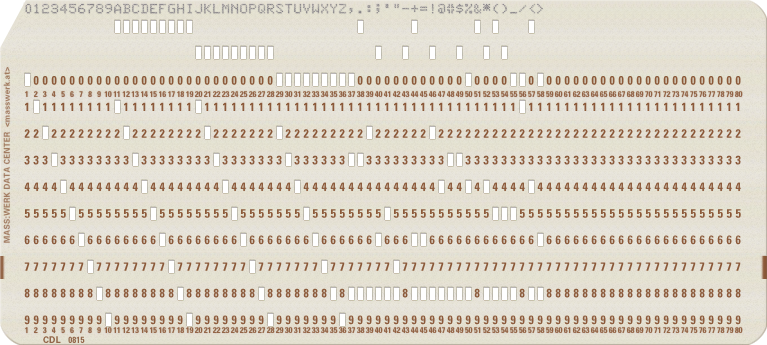
\includegraphics[width=\textwidth]{dkkp-1.png}
    \end{subfigure}    
    \caption{打孔卡片}
    \label{fig:dkkp-1}
\end{figure}

对于Fortran语言,打孔卡片的格式有一些特殊要求,称为Fortran的固定格式,每一行的要求如下:

\begin{center}

\begin{table}[!h]
        \centering
        
\begin{tabular}{|p{0.24\textwidth}|p{0.73\textwidth}|}
\hline 
 第1个字符 & 如果是字母C或*,这一行就是注释,不会被编译 \\
\hline 
 第1\textasciitilde 5个字符 & 如果是数字,就是给这一行代码取一个代号,不然只能是空格 \\
\hline 
 第6个字符 & 如果是“0”以外的任何字符,表示这一行程序接上一行 \\
\hline 
 第7\textasciitilde 72个字符 & Fortran程序代码的编写区域 \\
\hline 
 第73个字符及之后 & 保留区域,留空 \\
 \hline
\end{tabular}
        
        \end{table}
\end{center}

例如如下代码片段:
\begin{envcode}{fortran}{Fortran}
C THE FIRST FORTRAN PROGRAM
      WRITE(6,10)
   10 FORMAT(1X, 'HELLO, WORLD.')
      END
\end{envcode}
每一行在打孔卡片上就如图\ref{fig:dkkp-2}所示,每一行占一张卡片,共4张卡片。
(现在还不需要知道代码各个部分是什么意思,这里只是为了说明Fortran的固定格式和打孔卡片的概念。)

在向机器输入程序时,依次读取四张卡片即可。

\begin{figure}[h]
    \centering
    \captionsetup{font={small, bf}, margin=60pt}
    \begin{subfigure}[c]{0.48\textwidth}
      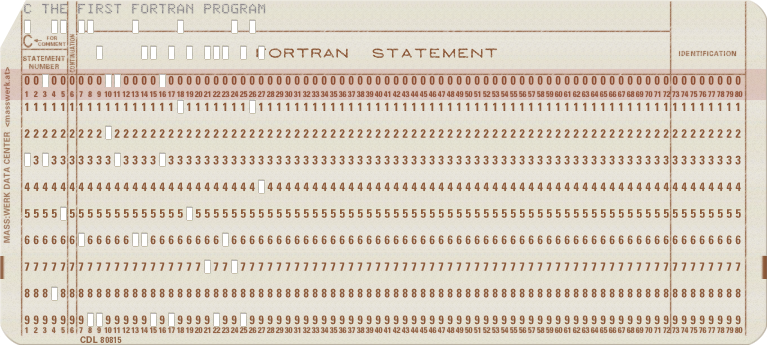
\includegraphics[width=\textwidth]{dkkp-2-1.png}
      \caption{第1行}
    \end{subfigure}
    \hfill
    \begin{subfigure}[c]{0.48\textwidth}
      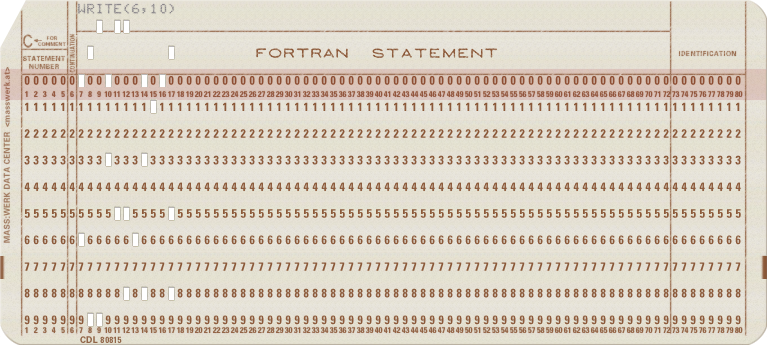
\includegraphics[width=\textwidth]{dkkp-2-2.png}
      \caption{第2行}
    \end{subfigure}
    \hfill
    \begin{subfigure}[c]{0.48\textwidth}
      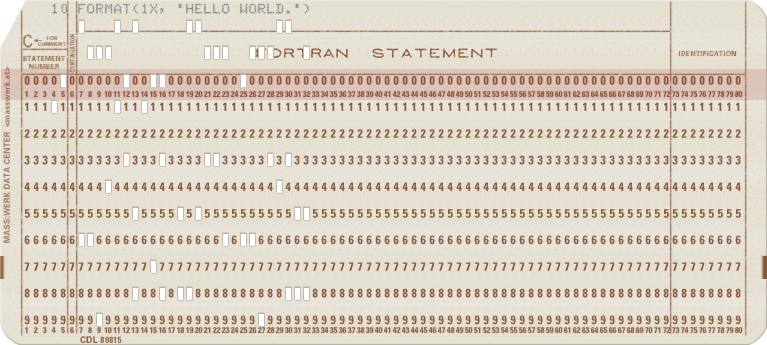
\includegraphics[width=\textwidth]{dkkp-2-3.png}
      \caption{第3行}
    \end{subfigure}
    \hfill
    \begin{subfigure}[c]{0.48\textwidth}
      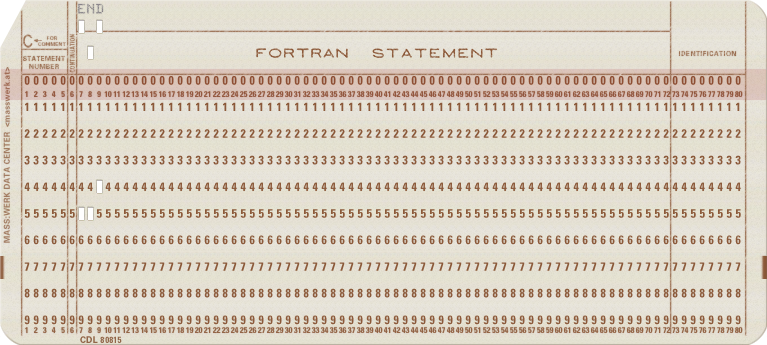
\includegraphics[width=\textwidth]{dkkp-2-4.png}
      \caption{第4行}
    \end{subfigure}    
    \caption{The first Fortran program}
    \label{fig:dkkp-2}
\end{figure}

整个程序编译后运行的输出结果为:
\begin{envcode}{text}{Text}
 HELLO, WORLD.
\end{envcode}

在打孔卡片上如图所示:
\begin{figure}[h]
    \centering
    \captionsetup{font={small, bf}, margin=60pt}
    \begin{subfigure}[c]{0.9\textwidth}
      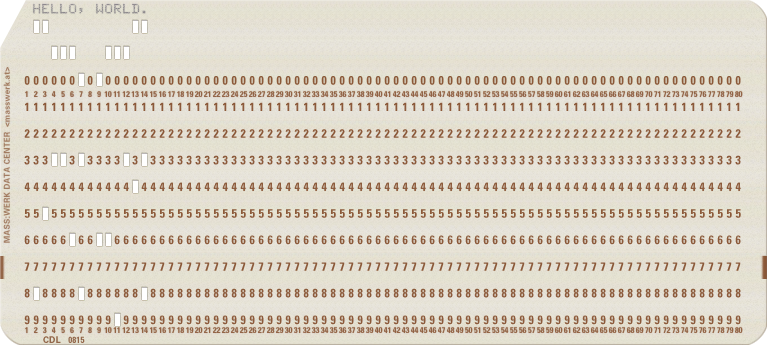
\includegraphics[width=\textwidth]{dkkp-3.png}
    \end{subfigure}    
    \caption{程序输出结果}
    \label{fig:dkkp-3}
\end{figure}

当然,现在已经没有人使用打孔卡片了,Fortran程序的编写和运行都可以在现代计算机上完成。
但是,Fortran的固定格式仍然保留了下来,Fortran程序的编写仍然需要遵循固定格式。

同时卡片的概念在Fortran中也保留了下来,
Fortran程序的每一行代码都可以看作是一张卡片,读取的每一行数据也可以看作是一张卡片。

另外,打孔卡片是不区分大小写的,Fortran程序的代码也不区分大小写。

\subsection{Fortran语言的编译}
Fortran程序需要经过编译器编译成机器语言才能被计算机执行。

在本笔记Linux部分已经提到了“gfortran”编译器的安装,如果还没有安装,可以使用以下命令安装:
\begin{envcode}{console}{Bash}
user1@host:~$ sudo apt-get install gfortran
\end{envcode}

以上面的例子为例,假设我们将代码保存在\code{learn}文件夹的\code{hello.f}:
\begin{envcode}{console}{Bash}
user1@host:~$ mkdir learn
user1@host:~$ cd learn
user1@host:~/learn$ vim hello.f
\end{envcode}

vim编辑器用法不再重复,在文件中写入上面例子的代码,注意按照固定格式确认好空格数:
\begin{envcode}{fortran}{Fortran}
C THE FIRST FORTRAN PROGRAM
      WRITE(6,10)
   10 FORMAT(1X, 'HELLO, WORLD.')
      END
\end{envcode}

保存并退出编辑器后,使用以下命令编译程序:
\begin{envcode}{console}{Bash}
user1@host:~/learn$ gfortran -c hello.f
user1@host:~/learn$ gfortran -o hello hello.o
user1@host:~/learn$ ls
hello  hello.f  hello.o
\end{envcode}

第一条命令会生成一个目标文件\code{hello.o},第二条命令会将目标文件链接成可执行文件\code{hello}。
运行程序使用以下命令:
\begin{envcode}{console}{Bash}
user1@host:~/learn$ ./hello
 HELLO, WORLD.
\end{envcode}

如果是像这样只有一个代码文件的简单程序,或者不想生成目标文件,可以直接使用以下命令编译并运行程序:
\begin{envcode}{console}{Bash}
user1@host:~/learn$ gfortran -o hello hello.f
user1@host:~/learn$ ./hello
 HELLO, WORLD.
\end{envcode}

这样不会生成目标文件\code{hello.o},直接生成可执行文件\code{hello}。

\newpage
\section{Fortran基础}
\subsection{Fortran变量类型声明与转化}
\subsubsection{Fortran变量类型声明}
Fortran语言中,变量的类型和声明是非常重要的概念。
Fortran支持多种数据类型,包括整数、实数(与数学上的实数定义不同)、字符等。

变量名可以包含字母、数字和下划线,但要以字母开头,同时不超过6个字符。

Fortran有隐式声明和显式声明两种方式。

隐式声明是指在使用变量之前不需要显式地声明变量的类型,Fortran会根据变量名的首字母自动推断类型,
例如以\code{I、J、K、L、M、N}开头的变量默认为整数类型,其它变量默认为实数类型。

显式声明是指在使用变量之前需要显式地声明变量的类型,使用类型声明语句,例如:
\begin{envcode}{fortran}{Fortran}
      INTEGER :: I
      REAL :: X
      DOUBLE PRECISION :: Y
\end{envcode}
上面第一行声明了一个整数类型的变量\code{I},第二行声明了一个单精度实数类型的变量\code{X},第三行声明了一个双精度实数类型的变量\code{Y}。

一般我们遵循隐式声明的规则,除非有特殊需要,否则不使用显式声明。

\subsubsection{Fortran变量类型转化}
Fortran语言中,变量类型的转化是一个重要的概念。Fortran提供了多种方式来进行变量类型的转化。

使用类型转换函数,例如:
\begin{envcode}{fortran}{Fortran}
      M = INT(A)
      N = IFIX(B)
      I = IDINT(C)
\end{envcode}
前两个语句将实数\code{A}和\code{B}转换为整数类型,第三个语句将双精度实数\code{C}转换为整数类型。可统一使用\code{INT}函数进行转换。

\begin{envcode}{fortran}{Fortran}
      X = REAL(I)
      Y = FLOAT(J)
      Z = DBLE(K)
\end{envcode}
前两个语句作用相同,将整数\code{I}和\code{J}转换为单精度实数类型,第三个语句将整数K转换为双精度实数类型。

以上可统一记为\code{INT}转化为整数,\code{REAL}转化为单精度实数,\code{DBLE}转化为双精度实数,其它的都能用这三个代替。

\subsection{Fortran程序的输入与输出}

Fortran程序的输入与输出主要通过以下几个语句实现:

\begin{itemize}
    \item \code{READ}:用于从标准输入设备(通常是键盘)读取数据。
    \item \code{WRITE}:用于向标准输出设备(通常是屏幕)输出数据。
    \item \code{PRINT}:用于向标准输出设备写入数据,语法更简单。
\end{itemize}

我们主要使用\code{READ}和\code{WRITE}语句来进行输入和输出。

\subsubsection{输入语句}

Fortran中的输入语句主要有两种形式:\code{READ}和\code{READ(*,*)}。

READ语句的基本形式为:
\begin{envcode}{fortran}{Fortran}
      READ, 变量
      READ(单位, 格式) 变量1 变量2 ...
\end{envcode}

其中,单位表示输入设备,其中\code{5}表示读卡器(在现代的电脑上就是用键盘输入),格式表示数据的格式,变量列表表示要读取的变量。

\code{READ(5,*)}表示从标准输入设备读取数据,格式由编译器自动推断,适用于简单的输入场景。

\subsubsection{输出语句}

Fortran中的输出语句主要有两种形式:\code{WRITE}和\code{PRINT}。


WRITE语句的基本形式为:
\begin{envcode}{fortran}{Fortran}
      WRITE(单位, 格式) 变量1 变量2 ...
\end{envcode}
其中,单位表示输出设备,其中\code{6}表示行式打印机(在现代的电脑上就是用屏幕输出),格式表示数据的格式,变量列表表示要输出的变量。

\texttt{PRINT}语句的基本形式为:
\begin{envcode}{fortran}{Fortran}
      PRINT(格式) 变量1 变量2 ...
\end{envcode}
    其中,格式表示数据的格式,变量列表表示要输出的变量。








\subsection{格式化输出}

Fortran支持格式化输入输出,可以通过格式字符串来控制输出的格式。
一般情况下,输入数据来源复杂,格式多样,我们会使用\code{*}表示自动推断格式;
输出时为了获取整齐美观的结果,可以指定格式。
下面只介绍输出的格式化,输入格式化类似,不再赘述。

\subsubsection{格式化输出语句}

上节命令如\code{READ}和\code{WRITE}中都有“格式”参数,一般读取时我们用\code{*}表示自动推断格式,
输出时我们可以指定格式。

指定格式有两种方式:

第一种是使用格式字符串,例如:
\begin{envcode}{fortran}{Fortran}
      WRITE(6, '(A, I5, F10.2, E10.2)') '结果是:', I, X
\end{envcode}
其中,\code{'(A, I5, F10.2, E10.2)'}表示输出一个字符串(A),一个整数(I5,宽度为5),一个单精度实数(F10.2,宽度为10,小数点后保留2位),一个双精度实数(E10.2,宽度为10,小数点后保留2位)。

第二种是使用格式标签,例如:
\begin{envcode}{fortran}{Fortran}
      WRITE(6, 100) I, X
  100 FORMAT('结果是:', I5, F10.2, E10.2)
\end{envcode}
其中,\code{100}是标签,其指定的行中的\code{FORMAT}语句定义了格式。如果格式字符串较长,可以使用标签来分割,避免超出固定格式行长度限制。

\subsubsection{I型}
I型格式用于输出整数,格式为\code{Iw},其中\code{w}表示输出的宽度,
可以理解为给这个数据5个字符的空间,例如:
\begin{envcode}{fortran}{Fortran}
      M=12345
      N=123
      K=123456
      WRITE(6, '(I5)') M
      WRITE(6, '(I5)') N
      WRITE(6, '(I5)') K
      END
\end{envcode}
编译后运行输出结果为:
\begin{envcode}{text}{Text}
12345
  123
*****
\end{envcode}
其中,\code{*****}表示输出的整数超过了指定的宽度,Fortran会用星号填充。

\subsubsection{F型}
F型格式用于输出单精度实数,格式为\code{Fw.d},
其中\code{w}表示输出的宽度,\code{d}表示小数点后保留的位数,
例如:
\begin{envcode}{fortran}{Fortran}
      K=1234567890
      X=123.456
      WRITE(6, '(I10)') K
      WRITE(6, '(F10.2)') X
      END
\end{envcode}
编译后运行输出结果为:
\begin{envcode}{text}{Text}
1234567890
    123.46
\end{envcode}
(这里第一行的整数用来标记位置,便于直观观察F型所占空间)
其中,\code{123.46}表示输出的单精度实数,Fortran会根据指定的格式进行填充和舍入。

\subsubsection{E型}
E型格式用于输出双精度实数,格式为\code{Ew.d},
其中\code{w}表示输出的宽度,\code{d}表示小数点后保留的位数,
例如:
\begin{envcode}{fortran}{Fortran}
      K=1234567890
      Y=-123.456
      Z=123.456
      WRITE(6, '(I10)') K
      WRITE(6, '(E10.3)') Y      
      WRITE(6, '(E10.3)') Z
      END
\end{envcode}
编译运行后输出结果为:
\begin{envcode}{text}{Text}
1234567890
-0.123E+03
 0.123E+03
\end{envcode}
(这里第一行的整数用来标记位置,便于直观观察E型所占空间)
其中,\code{0.123E+03}表示输出的双精度实数。

Fortran中标准的E型格式需要注意,一个数用科学计数法表示为\code{A*10^N},
表示为E型为\code{AEN},标准化E型中,A的整数部分为\code{0}。
如\code{123.456},则表示为\code{0.123456E+03}而不是\code{1.23456E+02},再根据格式进行填充和舍入。

以上内容可见,E型占用的空间较大,使用时注意前后留足空间,如使用\code{E20.5}。



\subsection{数学语句}

\subsubsection{数字与运算符}

在编写Fortran程序时,我们需要使用数字和运算符来进行计算。
整数如\code{123}、\code{-456}等,直接表示即可。

实数如\code{3.14}、\code{-2.718}等,直接表示即可;
\code{0.123}、\code{456.0},可以省略0,直接写为\code{.123}、\code{456.}。

Fortran常用的运算符有加(\code{+})、减(\code{-})、乘(\code{*})、除(\code{/})和幂(\code{**})等。
可直接对数字或变量进行运算。
运算优先级从高到低依次为:幂、乘除、加减。如果有括号,则括号内的运算优先级最高。

\subsubsection{数学函数}
Fortran提供了多种数学函数,用于对数字进行处理和计算。
例如:
\begin{envcode}{fortran}{Fortran}
      A = ABS(X)       ! 绝对值
      B = SQRT(Y)      ! 平方根
      C = EXP(Z)       ! 指数函数
      D = LOG(W)       ! 自然对数
      E = LOG10(V)     ! 常用对数
      F = SIN(T)       ! 正弦函数
      G = COS(U)       ! 余弦函数
      M = MAX(A, B)    ! 最大值
      N = MIN(C, D)    ! 最小值
      O = MOD(P, Q)    ! 取模
\end{envcode}

其中自然对数函数在课堂上介绍的是\code{ALOG},这是Fortran 77的函数,用于处理单精度实数;
另外还有\code{DLOG}用于处理双精度实数、\code{CLOG}用于处理复数,比较复杂。

在Fortran 90中,增加了\code{LOG}函数,包括了上面三种用法,兼容性强,推荐使用。

\subsubsection{赋值语句}
赋值语句用于将一个值赋给一个变量,例如:
\begin{envcode}{fortran}{Fortran}
      I = 5
      X = 3.14
      Y = 2.718281828459045
\end{envcode}

\subsubsection{算术运算}
Fortran支持基本的算术运算,包括加法、减法、乘法、除法等,例如:
\begin{envcode}{fortran}{Fortran}
      Z = X + Y
      A = B - C
      D = E * F
      G = H / I
      J = K ** L
\end{envcode}

\subsubsection{大型算术表达式}
Fortran支持大型算术表达式,可通过嵌套多层括号、合理利用运算符的优先级来实现复杂的计算。
例如:
\begin{equation*}
      z = \frac{\mathrm{e}^{x+y}+\sin{x}+s^t}{\left|x\right| + \sqrt{y} - \lg(w)}
\end{equation*}
用Fortran的数学语句表示为:
\begin{envcode}{fortran}{Fortran}
      Z = (EXP(X+Y) + SIN(X) + S**T) / (ABS(X) + SQRT(Y) - LOG10(W))
\end{envcode}

为了防止语句过长违反固定格式,可拆开表示:
\begin{envcode}{fortran}{Fortran}
      P = EXP(X+Y) + SIN(X) + S**T
      Q = ABS(X) + SQRT(Y) - LOG10(W)
      Z = P / Q
\end{envcode}

\subsection{Fortran程序构成}
Fortran程序一般由以下几个部分构成:
\begin{itemize}
      \item 程序头:包括程序名、变量声明等。
      \item 主程序:包含程序的主要逻辑和计算部分。
      \item 子程序:可选部分,用于实现特定功能的代码块。
      \item 结束语句:标志程序的结束。
\end{itemize}
例如:
\begin{envcode}{fortran}{Fortran}
      PROGRAM HelloWorld
      INTEGER :: I
      REAL :: X, Y
      
      WRITE(6, '(A)') 'Hello, World!'
      
      I = 5
      X = 3.14
      Y = 2.718281828459045
      
      WRITE(6, '(I5, F10.2, E10.3)') I, X, Y
      
      END PROGRAM HelloWorld
\end{envcode}

其中第一行\code{PROGRAM HelloWorld}表示程序名为\code{HelloWorld},非必须,可以不写。

接下来是变量声明部分,使用\code{INTEGER}和\code{REAL}声明了整数和实数类型的变量,这里的内容实际上包含在隐式声明内了,可以不再显式声明。

\code{END}语句标志程序的结束,后面的\code{PROGRAM HelloWorld}表示程序名的结束,可以直接写\code{END}。


% \section{Fortran程序结构}
一般而言,程序的结构有顺序结构、选择结构和循环结构。
% \include{content/chapter5.tex}
% \include{content/chapter6.tex}
% \include{content/chapter7.tex}
% \include{content/chapter8.tex}
% \include{content/chapter9.tex}
% \include{content/chapter10.tex}
% \include{content/chapter11.tex}


\newpage

% 参考文献
% \nocite{*}
% \bibliographystyle{unsrt}
% \addcontentsline{toc}{section}{\refname}
% \bibliography{references.bib}

\begin{appendices}
    \renewcommand{\thesection}{\Alph{section}}

\section{更换软件源为清华大学镜像站}
\label{sec:appendix-ubuntu-mirror}

\subsection{Ubuntu 24.04.2 LTS 软件源配置}
如果是按照文章开始的方式安装的Ubuntu系统,安装的版本应当是24.04.2 LTS(长期支持版),
请确保版本是24.04.2。
可以通过以下命令查看当前系统版本:
\begin{envcode}{console}{Bash}
user1@host:~$ lsb_release -a
No LSB modules are available.
Distributor ID: Ubuntu
Description:    Ubuntu 24.04.2 LTS
Release:        24.04
Codename:       noble
\end{envcode}

运行如下命令,打开软件源配置文件:
\begin{envcode}{console}{Bash}
user1@host:~$ sudo vim /etc/apt/sources.list.d/ubuntu.sources
\end{envcode}

不断按“dd”删除原有内容,直到清空文件。

然后按“i”进入插入模式,粘贴以下内容:
\begin{envcode}{text}{Text}
Types: deb
URIs: https://mirrors.tuna.tsinghua.edu.cn/ubuntu
Suites: noble noble-updates noble-backports
Components: main restricted universe multiverse
Signed-By: /usr/share/keyrings/ubuntu-archive-keyring.gpg

# 默认注释了源码镜像以提高 apt update 速度,如有需要可自行取消注释
# Types: deb-src
# URIs: https://mirrors.tuna.tsinghua.edu.cn/ubuntu
# Suites: noble noble-updates noble-backports
# Components: main restricted universe multiverse
# Signed-By: /usr/share/keyrings/ubuntu-archive-keyring.gpg

# 以下安全更新软件源包含了官方源与镜像站配置,如有需要可自行修改注释切换
Types: deb
URIs: http://security.ubuntu.com/ubuntu/
Suites: noble-security
Components: main restricted universe multiverse
Signed-By: /usr/share/keyrings/ubuntu-archive-keyring.gpg

# Types: deb-src
# URIs: http://security.ubuntu.com/ubuntu/
# Suites: noble-security
# Components: main restricted universe multiverse
# Signed-By: /usr/share/keyrings/ubuntu-archive-keyring.gpg

# 预发布软件源,不建议启用

# Types: deb
# URIs: https://mirrors.tuna.tsinghua.edu.cn/ubuntu
# Suites: noble-proposed
# Components: main restricted universe multiverse
# Signed-By: /usr/share/keyrings/ubuntu-archive-keyring.gpg

# # Types: deb-src
# # URIs: https://mirrors.tuna.tsinghua.edu.cn/ubuntu
# # Suites: noble-proposed
# # Components: main restricted universe multiverse
# # Signed-By: /usr/share/keyrings/ubuntu-archive-keyring.gpg
\end{envcode}

按“Esc”键退出插入模式,然后输入“:wq”后回车保存并退出。

接下来,运行以下命令更新软件源列表:
\begin{envcode}{console}{Bash}
user1@host:~$ sudo apt-get update
\end{envcode}

\subsection{更早或更新版本软件源配置}

清华大学开源软件镜像站一般只有LTS版本的Ubuntu软件源,首先请确保自己系统为LTS版本。

访问\textbf{\textcolor{blue}{\href{https://mirrors.tuna.tsinghua.edu.cn/help/ubuntu/}{清华大学开源软件镜像站}}},
仔细阅读网页指导内容,仿照上例更改软件源配置。或自行查找相关教程,这里不作介绍。




\section{与Window宿主机共享文件夹}
\label{sec:appendix-ubuntu-shared-folder}

\subsection{WSL子系统}
作为Windows 下的子系统,WSL(Windows Subsystem for Linux)可以直接访问Windows宿主机的文件系统。

在WSL中,Windows的文件系统通常挂载在\code{/mnt/c}目录下。你可以通过以下命令访问Windows的C盘、D盘,注意大小写:
\begin{envcode}{console}{Bash}
user1@host:~$ cd /mnt/c
user1@host:/mnt/c$ ls
Users  Program Files  Program Files (x86)  Windows ...
user1@host:~$ cd /mnt/d
\end{envcode}

复制、移动操作方式与Linux系统相同,可以使用\code{cp}、\code{mv}等命令。

\subsection{虚拟机}
如果按照文章开始的方法,正确配置虚拟机VMware,可以通过虚拟机的共享文件夹功能来实现与宿主机的文件共享。

按照下图所示,在虚拟机设置中启用共享文件夹功能,并添加想要共享的文件夹(图\ref{fig:shared-folder-setup})。
\begin{figure}[h]
    \centering
    \captionsetup{font={small, bf}, margin=60pt}
    \begin{subfigure}[c]{0.6\textwidth}
      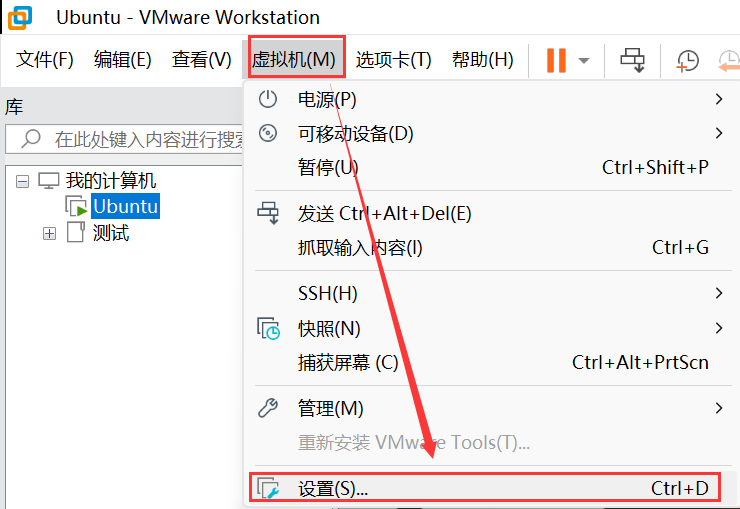
\includegraphics[width=\textwidth]{gxwjj-1.png}
    \end{subfigure}
    \hfill
    \begin{subfigure}[c]{0.35\textwidth}
      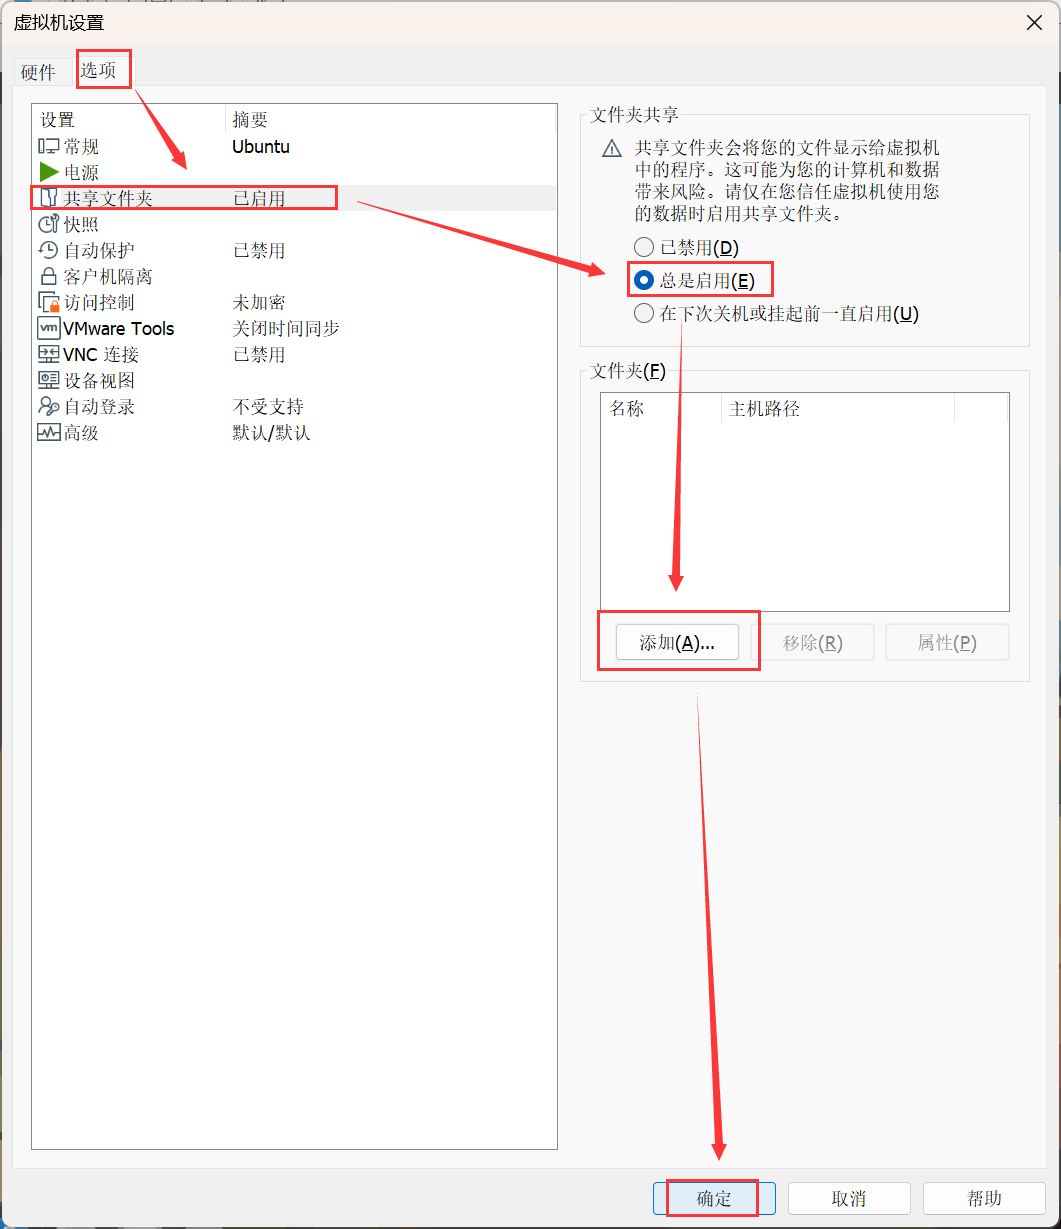
\includegraphics[width=\textwidth]{gxwjj-2.png}
    \end{subfigure}
    \caption{设置共享文件夹}
    \label{fig:shared-folder-setup}
\end{figure}

在“添加共享文件夹向导”的这一步时,点击“浏览”选择需要共享的文件夹,名称可不填(图\ref{fig:shared-folder-wizard})。
\begin{figure}[h]
    \centering
    \captionsetup{font={small, bf}, margin=60pt}
    \begin{subfigure}[c]{0.5\textwidth}
    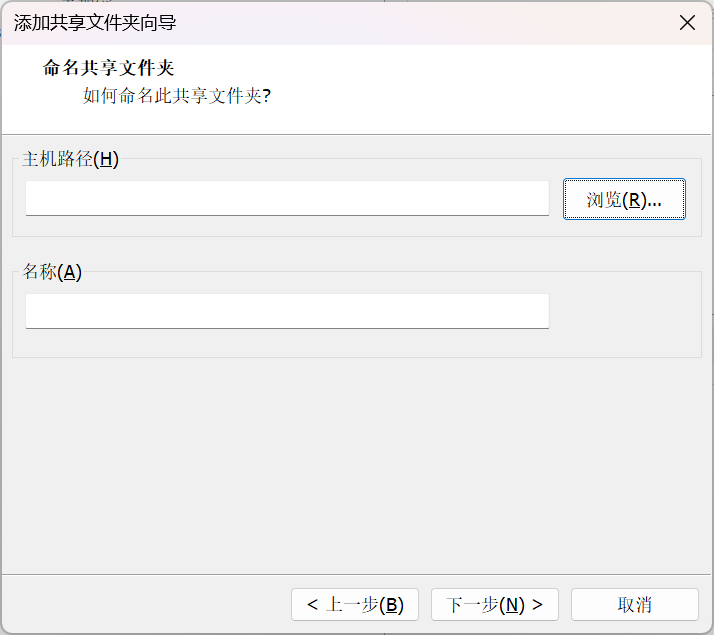
\includegraphics[width=\textwidth]{gxwjj-3.png}
    \end{subfigure}    
    \caption{共享文件夹向导}
    \label{fig:shared-folder-wizard}
\end{figure}

以上设置完成后,打开终端,运行以下命令:
\begin{envcode}{console}{Bash}
user1@host:~$ vmware-hgfsclient
\end{envcode}
若列出了所有共享的文件夹名称,则表示共享文件夹设置成功。

继续运行以下命令:
\begin{envcode}{console}{Bash}
user1@host:~$ sudo /usr/bin/vmhgfs-fuse .host:/ /mnt/hgfs -o allow_other -o uid=1000 -o gid=1000 -o umask=022
\end{envcode}
这将把共享文件夹挂载到\code{/mnt/hgfs}目录下。

现在,你可以通过以下命令访问共享文件夹:
\begin{envcode}{console}{Bash}
user1@host:~$ cd /mnt/hgfs
user1@host:/mnt/hgfs$ ls
SharedFolder1  SharedFolder2  ...
\end{envcode}
若显示了共享文件夹,则表示共享文件夹设置成功。

接下来设置开机自动挂载,
编辑\code{/etc/fstab}文件:
\begin{envcode}{console}{Bash}
user1@host:~$ sudo vim /etc/fstab
\end{envcode}

按\code{i}进入插入模式,移动光标到最后一行,
在文件末尾新建一行添加以下内容:
\begin{envcode}{text}{Text}
.host:/ /mnt/hgfs fuse.vmhgfs-fuse allow_other,uid=1000,gid=1000,umask=022 0 0
\end{envcode}

按\code{Esc}键退出插入模式,然后输入\code{:wq}后回车保存并退出。

重启虚拟机,进入\code{/mnt/hgfs}目录,如果可以看到共享的文件夹,则说明开机自动挂载设置成功。

如果需要访问共享文件夹,只需进入\code{/mnt/hgfs}目录即可。

如果之后需要添加新的共享文件夹,重复第一步,添加新的共享文件夹即可,不必重复设置开机自动挂载。


\end{appendices} 

\end{document}